\documentclass[a4paper,12pt,bibliography=totoc]{scrartcl}

\usepackage[utf8]{inputenc}
\usepackage[T1]{fontenc}
\usepackage[ngerman]{babel}
\usepackage{hyperref}
\usepackage{graphicx}
\usepackage[font=footnotesize]{caption}
\usepackage{subcaption}
\usepackage{amsthm,amsmath,amsfonts}

\title{Irgendwas mit Nummernschildern}
\author{Christian Peters}
\date{\today}

\setcounter{tocdepth}{2}

\begin{document}

\begin{titlepage}

    \maketitle

	\vfill

    \begin{tabular}{ll}
      Veranstaltung: & Fallstudien II \\
      Dozent: & Prof. Dr. Markus Pauly \\
      Gruppe: & Laura Kampmann, Christian Peters, Alina Stammen \\
    \end{tabular}
    
\thispagestyle{empty}
\end{titlepage}

\newpage
\tableofcontents
\thispagestyle{empty}

\newpage

\setcounter{page}{1}

\section{Einleitung}

Die automatisierte Erkennung von Nummernschildern aus Bilddaten
ist ein wichtiger Bestandteil vieler moderner Verkehrssysteme
und kommt beispielsweise in Parkh\"ausern, an Mautstellen
oder bei der Identifikation gestohlener Fahrzeuge zum
Einsatz~\cite{silva2018a}.

Das Ziel dieses Projektes ist es, einen Prototypen f\"ur ein solches
Erkennungssystem zu entwickeln, welcher in der
Lage sein soll, erfolgreich Nummernschilder aus Bilddaten erkennen
und auszulesen zu k\"onnen.

Zu diesem Zweck wird eine zweistufige Vorhersagepipeline konstruiert,
die ausgehend von einer Bilddatei im ersten Schritt den Bildausschnitt
bestimmt, der das Nummernschild enth\"alt, und im zweiten Schritt anhand
des zuvor ermittelten
Ausschnitts die Zeichen des Nummernschildes ausliest.

Bei der Bestimmung des relevanten Bildausschnittes, welcher das Nummernschild
enth\"alt, kommen sogenannte
Convolutional Neural Networks zum Einsatz, eine spezielle Art von
Neuronalen Netzen, deren Grundlagen in Abschnitt~\ref{sec:neuronale-netze}
beschrieben werden. Zum Auslesen der Zeichen werden die
Programmbibliotheken OpenCV~\cite{opencv_library} und
Tesseract~\cite{tesseract} verwendet.

Ein \"Uberblick \"uber das vorliegende Datenmaterial, welches
bei der Erstellung der Pipeline verwendet wurde, wird in
Abschnitt~\ref{sec:Datenbeschreibung} gegeben.
Der gesamte Aufbau der Pipeline wird in Abschnitt~\ref{sec:pipeline}
erl\"autert, im Anschluss werden die Ergebnisse in Abschnitt~\ref{sec:ergebnisse}
beschrieben und die St\"arken sowie die Schw\"achen des entwickelten
Prototypen diskutiert.

Der gesamte Quellcode dieses Projekts ist Open Source und kann
unter \url{https://github.com/cxan96/license_plate_detection}
abgerufen werden.


\section{Problemstellung}

\subsection{Datenbeschreibung}
\label{sec:daten}

Die vorliegenden Daten wurden im Zuge mehrerer Testfahrten durch das deutsche LTE-Netz der Netzbetreiber O2,
T-Mobile und Vodafone im Raum Dortmund erhoben~\cite{IEEE}.
Die Testfahrten verliefen \"uber vier zuvor festgelegte Routen, welche sich hinsichtlich der Art ihrer Umgebung unterscheiden:
\begin{itemize}
    \item \textbf{Campus}: Direkte Umgebung der TU Dortmund, Routenl\"ange 3km.
    \item \textbf{Urban}: Stadtbereich, Routenl\"ange: 3km.
    \item \textbf{Suburban}: Vorstadtbereich, Routenl\"ange: 9km.
    \item \textbf{Highway}: Autobahn, Routenl\"ange: 14km.
\end{itemize}
Jede dieser Messfahrten wurde zehnmal wiederholt.
Hierbei wurden sowohl passive Messungen der Netzqualit\"at mithilfe verschiedener Indikatoren, als auch aktive
Messungen der Up- und Downloadraten durchgef\"uhrt.
Die Messungen der Da\-ten\-\"uber\-tra\-gungs\-ra\-ten wurden alle 10s vollzogen, die Messungen der passiven Indikatoren alle 1s.
Um die Da\-ten\-\"uber\-tra\-gungs\-ra\-ten erfassen zu k\"onnen,
wurden Datenpakete zuf\"alliger Gr\"o{\ss}e von \mbox{0.1, 0.5, 1, ..., 10 MB} an einen Server zur Messung \"ubertragen.
Die insgesamt erhobenen Variablen seien in der folgenden Auflistung kurz beschrieben:
\begin{itemize}
    \item \textbf{RSRP:} \textit{Reference Signal Received Power} gibt die Empfangsst\"arke eines Referenzsignals an. Je h\"oher der Wert,
        desto besser ist der Empfang.
    \item \textbf{RSRQ:} \textit{Reference Signal Received Quality} ist ein weiterer Indikator f\"ur die Verbindungsqualit\"at.
        Er wird unter anderem aus dem RSRP berechnet und kann vom Funkmast verwendet werden, 
        um die Notwendigkeit eines Funkmastwechsels absch\"atzen zu k\"onnen.
    \item \textbf{SINR:} \textit{Signal-to-interference-plus-noise Ratio} gibt das Verh\"altnis des tats\"achlichen Signals zum Rauschen
        oder anderen St\"oreinfl\"ussen an.
    \item \textbf{CQI:} \textit{Channel Quality Indicator} ist ein Indikator, welcher Aufschluss \"uber die
        Qualit\"at des \"Ubertragungskanals gibt.
    \item \textbf{TA:} \textit{Timing Advance} gibt den Zeitversatz an, der zur Synchronisation zwischen Up- und Downlink
        verwendet wird. Damit gibt er indirekt Aufschluss \"uber die Entfernung zum Funkmast.
    \item \textbf{f:} Gibt die \textit{Frequenz} des LTE-Signals an.
    \item \textbf{Velocity:} Die Geschwindigkeit, mit der sich das Messger\"at fortbewegt.
    \item \textbf{Cell ID:} Identifiziert eine Zelle im LTE-Netzwerk. Nicht zu verwechseln mit der eNodeB-ID, welche einen Funkmast
        identifiziert. Ein Funkmast kann mehrere Zellen haben.
    \item \textbf{Payload Size:} Die Gr\"o{\ss}e des \"ubertragenen Datenpakets zur Ermittlung der Daten\"ubertragungsrate.
    \item \textbf{Data Rate:} Die gemessene Daten\"ubertragungsrate. Es werden sowohl Upload- als auch Downloadraten gemessen.
\end{itemize}

Die Messungen aller Testfahrten lassen sich insgesamt zu vier verschiedenen Datens\"atzen zusammenfassen, welche auch sp\"ater
zur Bearbeitung der Projektziele verwendet werden:
\begin{itemize}
    \item \textbf{Context}: Dieser Datensatz enth\"alt die sek\"undlich durchgef\"uhrten passiven Messungen der Netzwerkindikatoren.
        Insgesamt enth\"alt dieser Datensatz 68334 Messungen.
    \item \textbf{Cells}: Enth\"alt Messungen des RSRP und RSRQ zu den Nachbarzellen der aktuell verbundenen Zelle.
        Dieser Datensatz enth\"alt insgesamt 93443 Messungen.
    \item \textbf{Upload}: Dieser Datensatz enth\"alt die Messungen der Upload-Raten, welche alle 10s durchgef\"uhrt werden zuz\"uglich
        der Indikatoren aus dem Context-Datensatz zum entsprechenden Zeitpunkt. Insgesamt enth\"alt dieser Datensatz 6180 Messungen.
    \item \textbf{Download}: Analog zum Upload-Datensatz, nur dass hier die gemessenen Down\-load-Ra\-ten erfasst wurden.
        Dieser Datensatz enth\"alt insgesamt 6516 Messungen.
\end{itemize}

\subsection{Zielsetzungen}

\subsubsection{Task I -- Vorhersage der Daten\"ubertragungsraten}

In~\cite{IEEE} wurde ein neuartiger Ansatz der datengetriebenen Simulation von Netzwerken
(Data-driven Network Simulation, \textit{DDNS}) vorgestellt, welcher darauf basiert, dass durch datengetriebene Modelle m\"oglichst
realit\"atsnahe Simulationen von Netzwerken erzeugt werden sollen.
Ein Aspekt dieser Modelle besteht darin, dass Up- und Down\-load\-ra\-ten abh\"angig von den \"ubrigen Netzwerkindikatoren 
m\"oglichst realistisch modelliert werden m\"ussen.
Hierzu werden Pr\"adiktionsmodelle ben\"otigt, welche diese Da\-ten\-\"uber\-tra\-gungs\-ra\-ten entsprechend vorhersagen k\"onnen.

Das erste Ziel dieses Projektes ist es nun, verschiedene Arten von Pr\"a\-dik\-tions\-mo\-dellen im Hinblick auf diese Problemstellung
an\-zu\-wen\-den, und die G\"ute dieser Verfahren zu untersuchen.
Hierbei wird auch analysiert, ob sich das Verhalten der Modelle bez\"uglich der verschiedenen Netzbetreiber und Testfahrtszenarien
unterscheidet.
Weiterhin wird auch die Relevanz der verwendeten Kovariablen untersucht.

\subsubsection{Task II -- Vorhersage der eNodeB-Verbindungsdauern}

Bei den ersten Eins\"atzen von DDNS in~\cite{IEEE} hat sich gezeigt, dass es oft zu gro{\ss}en Vorhersagefehlern kommt, wenn der
Funkmast gewechselt wird (in der Fachsprache hei{\ss}en LTE-Funkmasten auch \textit{eNodeB}).
Eine Idee, um diesem entgegenzuwirken ist, den Zeitpunk des eNodeB-Wechsels vorherzusagen. Kennt man diesen Zeitpunkt, k\"onnte man
diese Information im n\"achsten Schritt dazu verwenden, um die Pr\"adiktionsmodelle zu verbessern.

Das zweite Ziel dieses Projektes ist also, die Restdauer der bestehenden Verbindung zu einer eNodeB und damit indirekt auch den
Wechselzeitpunk zur n\"achsten eNodeB vorherzusagen.
Auch hier wird die G\"ute des eingesetzten Pr\"adiktionsmodells anschlie{\ss}end analysiert und das Verhalten des Modells bez\"uglich
der verschiedenen Netzbetreiber und Einsatzszenarien, sowie die Relevanz der verwendeten Kovariablen untersucht.


\section{Methodik}

\subsection{Allgemeine Vorgehensweise}

\subsubsection{Vorhersage der Daten\"ubertragungsraten}

Die Vorhersage der Daten\"ubertragungsraten wird analog zu~\cite{IEEE} ebenfalls mithilfe von
Pr\"adiktionsmodellen aus dem Bereich des Machine-Learning bzw. des statistischen Lernens vorgenommen.
Hierbei kommen die Verfahren \textit{Extreme Gradient Boosting} und \textit{Lineare Regression mit ARMA-Fehlern}
zum Einsatz, welche in den Abschnitten~\ref{sec:xgboost} und~\ref{sec:arma} n\"aher beschrieben werden.
Analog zu~\cite{IEEE} wird auch hier f\"ur jeden Netzbetreiber ein eigenes Modell angepasst.

Der in Abschnitt~\ref{sec:daten} beschriebene Upload Datensatz, welcher s\"amtliche Kovariablen und die Zielvariable
\textit{Data Rate} enth\"alt, dient hierbei als Basis zur Vorhersage der Upload-Datenraten.
Analog dient der Download Datensatz zur Pr\"adiktion der Download Datenraten.
In beiden F\"allen werden die Modelle also so angepasst, dass sie basierend auf den Kovariablen, also der gemessenen Netzwerkindikatoren,
die Zielvariable \textit{Data Rate} prognostizieren sollen.

\subsubsection{Vorhersage der eNodeB-Verbindungsdauern}

Zur Vorhersage der Verbindungsdauern zu einer eNodeB kommen neben den Messungen zur aktuellen LTE-Zelle auch Messungen
zu den Nachbarzellen in Betracht. In diesem Fall liegen f\"ur die Nachbarzellen Messungen des RSRP sowie des RSRQ vor,
welche sich im Cells Datensatz finden. Der Context Datensatz enth\"ahlt alle Messungen bez\"uglich der aktuell verbundenen
Zelle und soll als Basis f\"ur die Prognose der eNodeB-Verbindungsdauern dienen. Da dieser Datensatz aber keine Informationen
zu den Nachbarzellen enth\"alt, m\"ussen die Datens\"atze Context und Cells vor der Pr\"adiktion noch zusammengef\"uhrt werden.
Die eNodeB-IDs, welche zu diesem Zweck ben\"otigt werden, lassen sich unmittelbar aus der \textit{Cell ID} bestimmen.
Das Zusammenf\"uhren der Datens\"atze geschieht so,
dass zu jedem Zeitpunkt sowohl die Netzwerkindikatoren zur aktuell verbundenen eNodeB vorliegen, als auch die
Informationen zum h\"ochsten RSRP und RSRQ einer benachbarten eNodeB.
Der Gedankengang hierbei ist, dass eine steigende Signalst\"arke bei einer benachbarten eNodeB m\"oglicherweise Aufschluss \"uber einen
baldigen Verbindungswechsel geben k\"onnte.

Die Zielvariable, also die Restdauer der aktuellen Verbindung zu einer eNodeB, kann leicht aus den Messdaten berechnet werden,
indem man die Differenz des Zeitpunktes der aktuellen Messung zu dem Zeitpunkt der ersten zuk\"unftigen Messung an einer neuen
eNodeB bildet. Als Pr\"adiktionsmodell der Verbindungsdauern kommt dann erneut das \textit{Extreme Gradient Boosting} zum Einsatz,
welches f\"ur jeden der drei Netzbetreiber separat angepasst wird.

\subsubsection{Validierung und Tuning}
\label{sec:validierung-tuning}

Die Modellvalidierung erf\"ullt den Zweck, Aussagen dar\"uber treffen zu k\"onnen, wie sich die trainierten Modelle
auf neuen und ungesehenen Daten, also beispielsweise zuk\"unfig stattfindenden Messungen, 
verhalten werden.
Ein bekanntes Verfahren dazu ist die $k$-fache Kreuzvalidierung~\cite{elements}, welche auch in~\cite{IEEE} zum Einsatz
gekommen ist.
Hierbei wird der gesamte Datensatz zun\"achst zuf\"allig in $k$ gleich gro{\ss}e Partitionen unterteilt,
um im Anschluss das Modell jeweils auf $k-1$ Partitionen
zu trainieren und die \"ubrige Partition zum testen zu verwenden. Dies wird solange wiederholt, bis jede der
$k$ Partitionen genau einmal zum testen verwendet wurde.
Obwohl dieses Verfahren sehr weit verbreitet ist, gibt es in der vorliegenden Situation jedoch Anhaltspunkte daf\"ur,
dass sich die $k$-fache Kreuzvalidierung m\"oglicherweise als problematisch erweisen k\"onnte.

In Abbildung~\ref{fig:messfahrt-vodafone} ist eine der durchgef\"uhrten Messfahrten einmal beispielhaft zu sehen.
Man erkennt sofort, dass es sich bei den gemessenen Daten offenbar um eine Zeitreihe handelt.
W\"urde man in dieser Situation eine $k$-fache Kreuzvalidierung einsetzen, bei der die Daten zuf\"allig partitioniert werden,
so w\"urde der zeitliche Zusammenhang zwischen den Beobachtungen dadurch verloren gehen.
Es w\"are also fraglich, ob durch diese Art der Validierung verl\"assliche Aussagen \"uber das Modellverhalten auf zuk\"unftig
erhobenen Messdaten getroffen werden k\"onnen.
Aus diesem Grund wurde in diesem Projekt ein eigenes Validierungsverfahren eingesetzt, welches speziell auf die vorliegende Situation
zugeschnitten wurde.

\begin{figure}
    \centering
    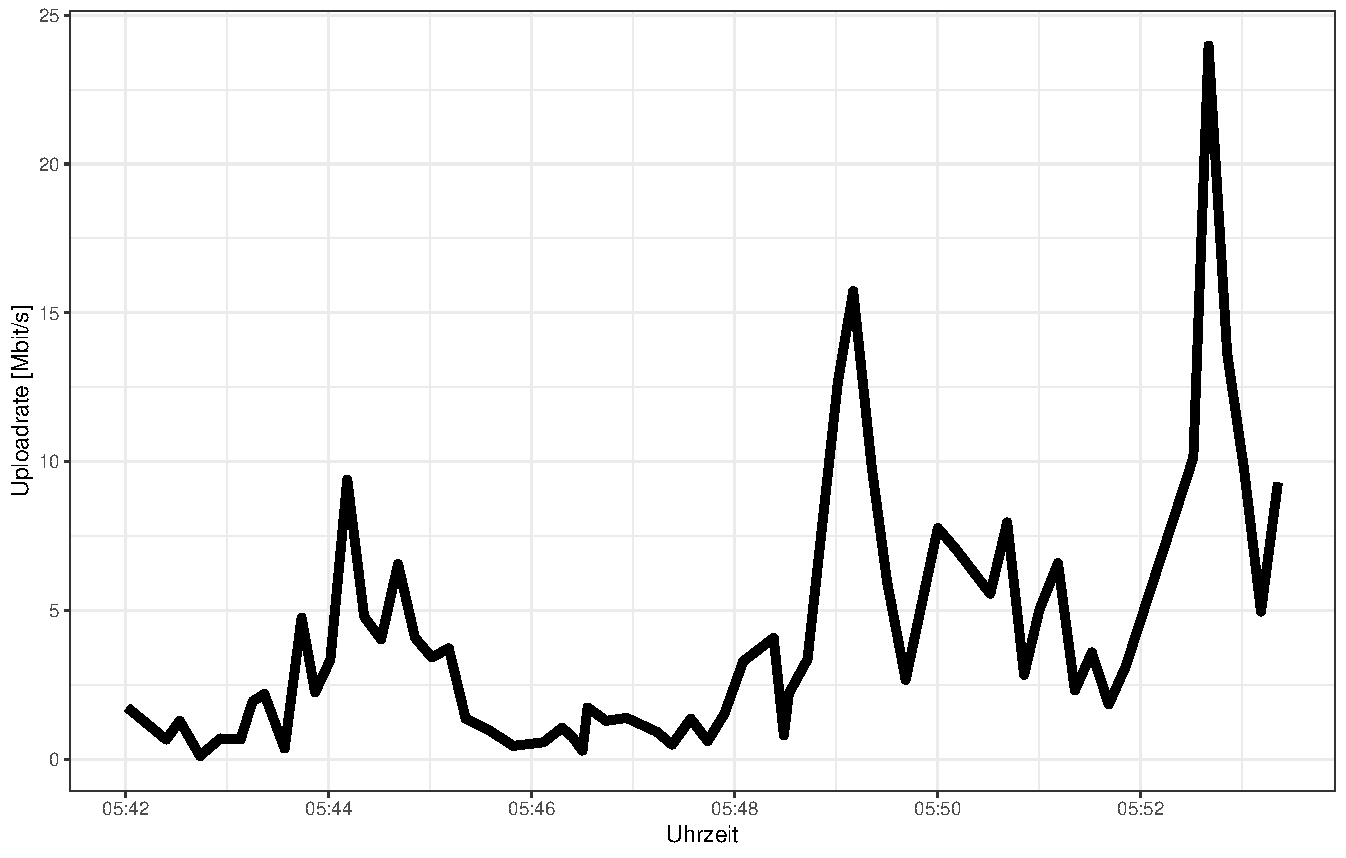
\includegraphics[width=0.8\textwidth]{abbildungen/highway_drive_vodafone}
    \caption{Die erste Messfahrt auf der Autobahn f\"ur den Netzbetreiber Vodafone am 12.12.2018.}
    \label{fig:messfahrt-vodafone}
\end{figure}

In Abbildung~\ref{fig:validierung} ist die in diesem Projekt eingesetzte Validierungsmethode einmal schematisch dargestellt.
Wie bereits beschrieben, besteht der gesamte Datensatz an Messungen f\"ur einen Netzbetreiber aus zehn einzelnen Messfahrten f\"ur
jedes der Szenarien \textit{campus}, \textit{highway}, \textit{suburban} und \textit{urban}.
Jeder dieser Fahrten kann also chronologisch eine Nummer von 1-10 zugewiesen werden, welche zusammen mit dem Szenario
eine Fahrt eindeutig identifiziert.
Im hier eingesetzten Validierungsverfahren wurde nun zun\"achst der gesamte Datensatz in zwei Teile aufgeteilt.
Der erste Teil besteht aus den Fahrten 1-7, der zweite Teil besteht aus den Fahrten 8-10.
In der Trainingsphase und beim Parametertuning kommt ausschlie{\ss}lich der erste Teil der Fahrten 1-7 zum Einsatz.
So wird sichergestellt, dass das Modell beim Training keine Informationen aus zuk\"unftigen Fahrten mit einbeziehen kann, wie
es beispielsweise bei der $k$-fachen Kreuzvalidierung der Fall w\"are. Fahrten 8-10 werden also ausschlie{\ss}lich zur Modellvalidierung
eingesetzt.

\begin{figure}
    \centering
    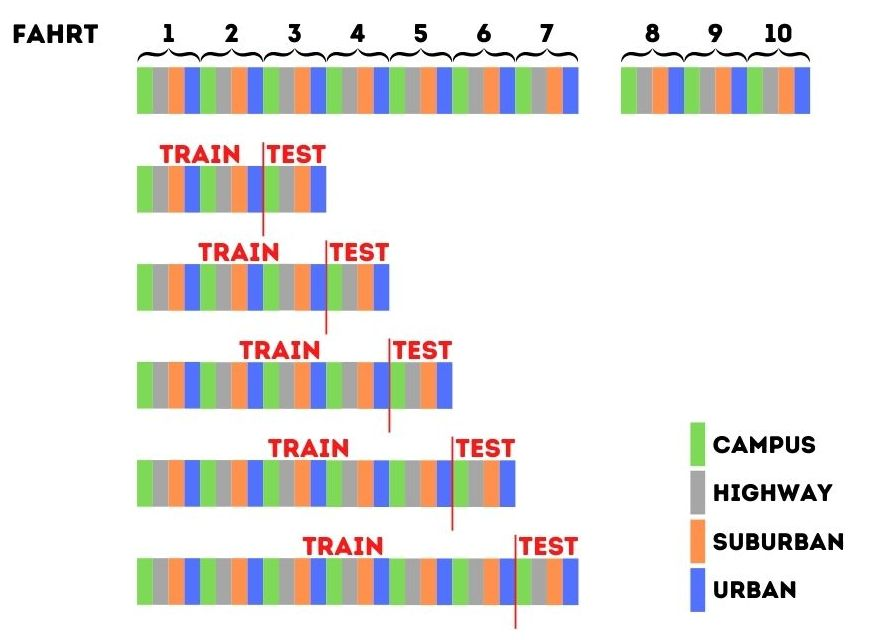
\includegraphics[width=0.8\textwidth]{abbildungen/validierung}
    \caption{Das eingesetzte Verfahren zur Modellvalidierung.}
    \label{fig:validierung}
\end{figure}

\paragraph{Kennzahlen zur Evaluation der Vorhersagequalit\"at}

Um die Vorhersagequalit\"at der eingesetzten Verfahren zu bewerten, werden die Kennzahlen
$R^2$, sowie der Mean Absolute Error (MAE) auf den Out-of-Sample Fahrten 8-10 wie folgt berechnet:
\begin{equation}
    R^2 = 1 - \frac{\sum_{i=1}^n \left( t_i - r_i \right)^2}{\sum_{i=1}^n \left( t_i - \bar{t} \right)^2}
\end{equation}
\begin{equation}
    \text{MAE} = \frac{1}{n} \sum_{i=1}^n \left| t_i - r_i \right|
\end{equation}
Hierbei ist $n$ die Anzahl der vorhergesagten Datenpunkte, $t_i$ gibt den wahren Wert der Zielgr\"o{\ss}e des $i$-ten Datenpunktes an,
$r_i$ gibt den vorhergesagten Wert f\"ur die Zielgr\"o{\ss}e des $i$-ten Datenpunktes an und $\bar{t}$ bezeichnet den Mittelwert der
Zielgr\"o{\ss}e.

\paragraph{Tuning der Hyperparameter}

Das Tuning der Hyperparameter wird systematisch auf den Fahrten 1-7 mithilfe einer zuf\"alligen Gittersuche vorgenommen.
Dabei wird f\"ur jedes Modell ein fester Suchraum der Hyperparameter definiert, welcher entlang jeder Dimension in feste
Gitterpunkte unterteilt wird. Das entstehende Gitter wird dann an einer festen Anzahl zuf\"alliger Stellen ausgewertet
und die zugeh\"origen Parameterkombinationen werden evaluiert.

Zur Evaluation einer Parameterkombination kommt, wie sich in Abbildung~\ref{fig:validierung} ebenfalls
erkennen l\"asst, eine Art Kreuzvalidierung f\"ur Zeitreihen zum Einsatz. Dabei wird der Trainingsdatensatz sukzessive um eine Fahrt
erweitert und es wird immer auf der n\"achsten Fahrt getestet.
Dies soll die Begebenheit simulieren, dass nach und nach neue Messfahrten
vorgenommen werden, die den Gesamtdatensatz Schritt f\"ur Schritt erweitern.

Als G\"utekriterium f\"ur eine getestete Parameterkombination wird der MAE verwendet. Die beste Kombination aus Hyperparametern
wird dann im Anschluss auf dem gesamten Trainingsdatensatz der Fahrten 1-7 zur Modellanpassung genutzt und anschlie{\ss}end
auf den Validierungsfahrten 8-10 evaluiert.

\subsection{Extreme Gradient Boosting}
\label{sec:xgboost}

Extreme Gradient Boosting ist ein Verfahren aus dem Bereich des maschinellen Lernens, welches sich
in den letzten Jahren einer immer gr\"o{\ss}eren Beliebtheit erfreut hat~\cite{XGBoost}.
Die Grundlegende Funktionsweise dieses Verfahrens sei im Folgenden kurz beschrieben.

\subsubsection{Ausgangssituation}

Wir gehen davon aus, dass wir \"uber einen Trainingsdatensatz $\mathcal{D} = \{(\mathbf{x}_i, y_i)\}$
der Gr\"o{\ss}e $\left| \mathcal{D} \right| = n$ verf\"ugen, welcher aus den beobachteten Messungen $\mathbf{x}_i \in \mathbb{R}^m$
und der Zielgr\"o{\ss}e $y_i \in \mathbb{R}$ besteht, deren Wert wir vorhersagen wollen.

Das Ziel des Tree Boosting ist es, den Wert von $y_i$ durch ein Ensemble von Entscheidungsb\"aumen (CART)
vorherzusagen:
\begin{equation}
    \hat{y_i} = \phi(\mathbf{x}_i) =  \sum_{k=1}^K f_k(\mathbf{x}_i), \quad f_k \in \mathcal{F}
\end{equation}
Hierbei ist $\mathcal{F}$ die Klasse der besagten Entscheidungsb\"aume, welche in jedem ihrer $T$ Bl\"atter
einen konstanten Wert vorhersagen: $\mathcal{F} = \{f(\mathbf{x}) = w_{q(x)}\}$, wobei $q: \mathbb{R}^m \rightarrow T$
eine Funktion ist, die der Beobachtung $\mathbf{x}$ eines der $T$ Bl\"atter zuordnet und $w \in \mathbb{R}^T$ der Vektor
der Blattvorhersagen (Gewichte) des Baumes ist.

\subsubsection{Zielfunktion}

Die Zielfunktion, welche w\"ahrend des Trainings zur Anpassung des Modells minimiert wird, setzt sich wie folgt zusammen:
\begin{equation}
    \mathcal{L}(\phi) = \sum_{i=1}^n l(\hat{y}_i, y_i) + \sum_{k=1}^K \Omega(f_k)
\end{equation}
Hierbei ist $l$ eine differenzierbare und konvexe Verlustfunktion, welche Aufschluss \"uber die G\"ute der Vorhersage $\hat{y}_i$
liefert. Ein Beispiel ist der quadratische Fehler, welcher durch $l(\hat{y}_i, y_i) = (\hat{y}_i - y_i)^2$ gegeben ist.
Die Funktion $\Omega$ ist ein sogenannter Regularisierungs- oder Strafterm und ist wie folgt definiert:
\begin{equation}
    \Omega(f) = \gamma T + \frac{1}{2} \lambda \left \lVert w \right \rVert^2
\end{equation}
Das Ziel von $\Omega$ ist es, eine zu hohe Komplexit\"at der einzelnen Entscheidungsb\"aume in der Optimierung zu bestrafen und somit
w\"ahrend des Trainings simplere B\"aume zu bevorzugen. Dies geschieht mit dem Hintergedanken, eine \"Uberanpassung des Modells an
die Trainingsdaten verhindern zu wollen.
Der Parameter $\gamma$ bestraft hierbei die Anzahl der Bl\"atter $T$ eines Entscheidungsbaumes und der Parameter $\lambda$ bestraft
zu gro{\ss}e Gewichte in den einzelnen Bl\"attern.

\subsubsection{Training}

Das Grundprinzip des Boosting ist es, die Ensemble Modelle additiv nach dem Greedy-Prinzip zu trainieren.
Dies funktioniert hier so, dass die einzelnen Entscheidungsb\"aume nicht alle gleichzeitig angepasst werden, sondern
nach und nach zum Ensemble hinzugef\"ugt werden. Jeder Baum, welcher in einem Schritt hinzugef\"ugt wird, wird so trainiert,
dass er die Zielfunktion soweit wie m\"oglich minimiert.

Wenn im Optimierungsschritt $t$ also der Entscheidungsbaum $f_t$ zum Ensemble hinzugef\"ugt wird, ergibt sich die folgende
Verlustfunktion, welche durch $f_t$ minimiert werden soll:
\begin{equation}
    \mathcal{L}^{(t)} = \sum_{i=1}^n l(\hat{y}^{(t-1)}_i + f_t(\mathbf{x}_i), y_i) + \Omega(f_t)
\end{equation}
Die Regularisierungsterme $\sum_{k=1}^{t-1} \Omega(f_k)$ der bereits zum Ensemble hinzugef\"ugten B\"aume wurden hierbei weggelassen,
da sie im Zuge der Optimierung in Schritt $t$ nicht mehr ver\"andert werden k\"onnen.

Beim Extreme Gradient Boosting wird $\mathcal{L}^{(t)}$ nun im Punkt $\hat{y}^{(t-1)}_i$ durch ein Taylor-Polynom 2. Grades
approximiert, welches sich analytisch minimieren l\"asst.
Streicht man alle konstanten Terme, welche f\"ur die Minimierung keine Rolle spielen, erh\"alt man so die folgende Taylor-Approximation:
\begin{equation}
    \tilde{\mathcal{L}}^{(t)} = \sum_{i=1}^{n} \left[ g_i f_t(x_i) + \frac{1}{2}h_i f_t^2(x_i) \right] + \Omega(f_t)
\end{equation}
Hierbei sind $g_i = \partial_{\hat{y}_i^{(t-1)}} l(y_i, \hat{y}_i^{(t-1)})$ und 
$h_i = \partial_{\hat{y}_i^{(t-1)}}^2 l(y_i, \hat{y}_i^{(t-1)})$ die erste und zweite partielle Arbleitung der Verlustfunktion
$l$.

Wie in~\cite{XGBoost} gezeigt wurde, lassen sich dann die optimalen Gewichte $w_j^*, j=1 \ldots T$ f\"ur eine gegebene Baumstruktur
$q$ durch analytische Minimierung von $\tilde{\mathcal{L}}^{(t)}$ berechnen.
Die Bestimmung einer optimalen Baumstruktur $q$ hingegen ist rechnerisch durch Enumeration aller erdenklichen M\"oglichkeiten im
Normalfall keine Option.
Daher wird analog zum CART-Algorithms ein Greedy-Verfahren eingesetzt, welches den Baum durch sukzessives Hinzuf\"ugen neuer
Verzweigungen aufbaut.
Jede neue Verzweigung wird dabei so gew\"ahlt, dass der Wert von $\tilde{\mathcal{L}}^{(t)}$ durch die Bestimmung der optimalen
Gewichte zum aktuellen Baum soweit wie m\"oglich minimiert wird.
Der Regularisierungsterm $\Omega(f_t)$ verhindert dabei direkt durch seine Anwesenheit in $\tilde{\mathcal{L}}^{(t)}$, dass die neue
Baumstruktur zu komplex wird.

\subsubsection{Hyperparameter}

Die Hyperparameter des Extreme Gradient Boosting, welche im Rahmen dieses Projektes durch Tuning
ermittelt wurden, seien im Folgenden kurz aufgelistet:
\begin{itemize}
    \item $n$: Anzahl der Boosting-Runden und damit auch Anzahl der B\"aume, die insgesamt zum Ensemble hinzugef\"ugt werden.
        Je gr\"o{\ss}er dieser Parameter gew\"ahlt wird, desto komplexer wird das Modell.
    \item $\gamma$: Regularisierungsterm, welcher die Anzahl an Bl\"attern eines Entscheidungsbaumes bestraft.
        Dies soll die Bildung von zu komplexen B\"aumen im Ensemble verhindern und somit eine Ma{\ss}nahme gegen potenzielle
        \"Uberanpassung sein.
    \item $\lambda$: Bestraft zu hohe Gewichte in den Bl\"attern eines Entscheidungsbaumes, wird ebenfalls zur Vermeidung von
        \"Uberanpassung verwendet.
    \item $\eta$: Wurde in einer Boosting-Runde ein neuer Baum gefunden, so geht er nur mit dem Gewicht $\eta$ in das 
        Gesamtensemble ein. Dies ist eine weitere Ma{\ss}nahme, die gegen \"Uberanpassung des Modells helfen soll.
\end{itemize}
Der Suchraum, welcher im Tuningprozess zur Ermittlung einer m\"oglichst guten Kombination der Hyperparameter verwendet wurde, 
sei ebenfalls hier angegeben:
\begin{itemize}
    \item $n \in \left[100, 1000 \right]$
    \item $\gamma \in \left[0, 10 \right]$
    \item $\lambda \in \left[0, 10 \right]$
    \item $\eta \in \left[0.01, 1 \right]$
\end{itemize}

\subsection{Lineare Regression mit ARMA-Fehlern}
\label{sec:arma}


\section{Ergebnisse}

\subsection{Vorhersage der Daten\"ubertragungsraten}

\subsubsection{Extreme Gradient Boosting}

\begin{figure}
\centering
\begin{subfigure}{\textwidth}
    \centering
    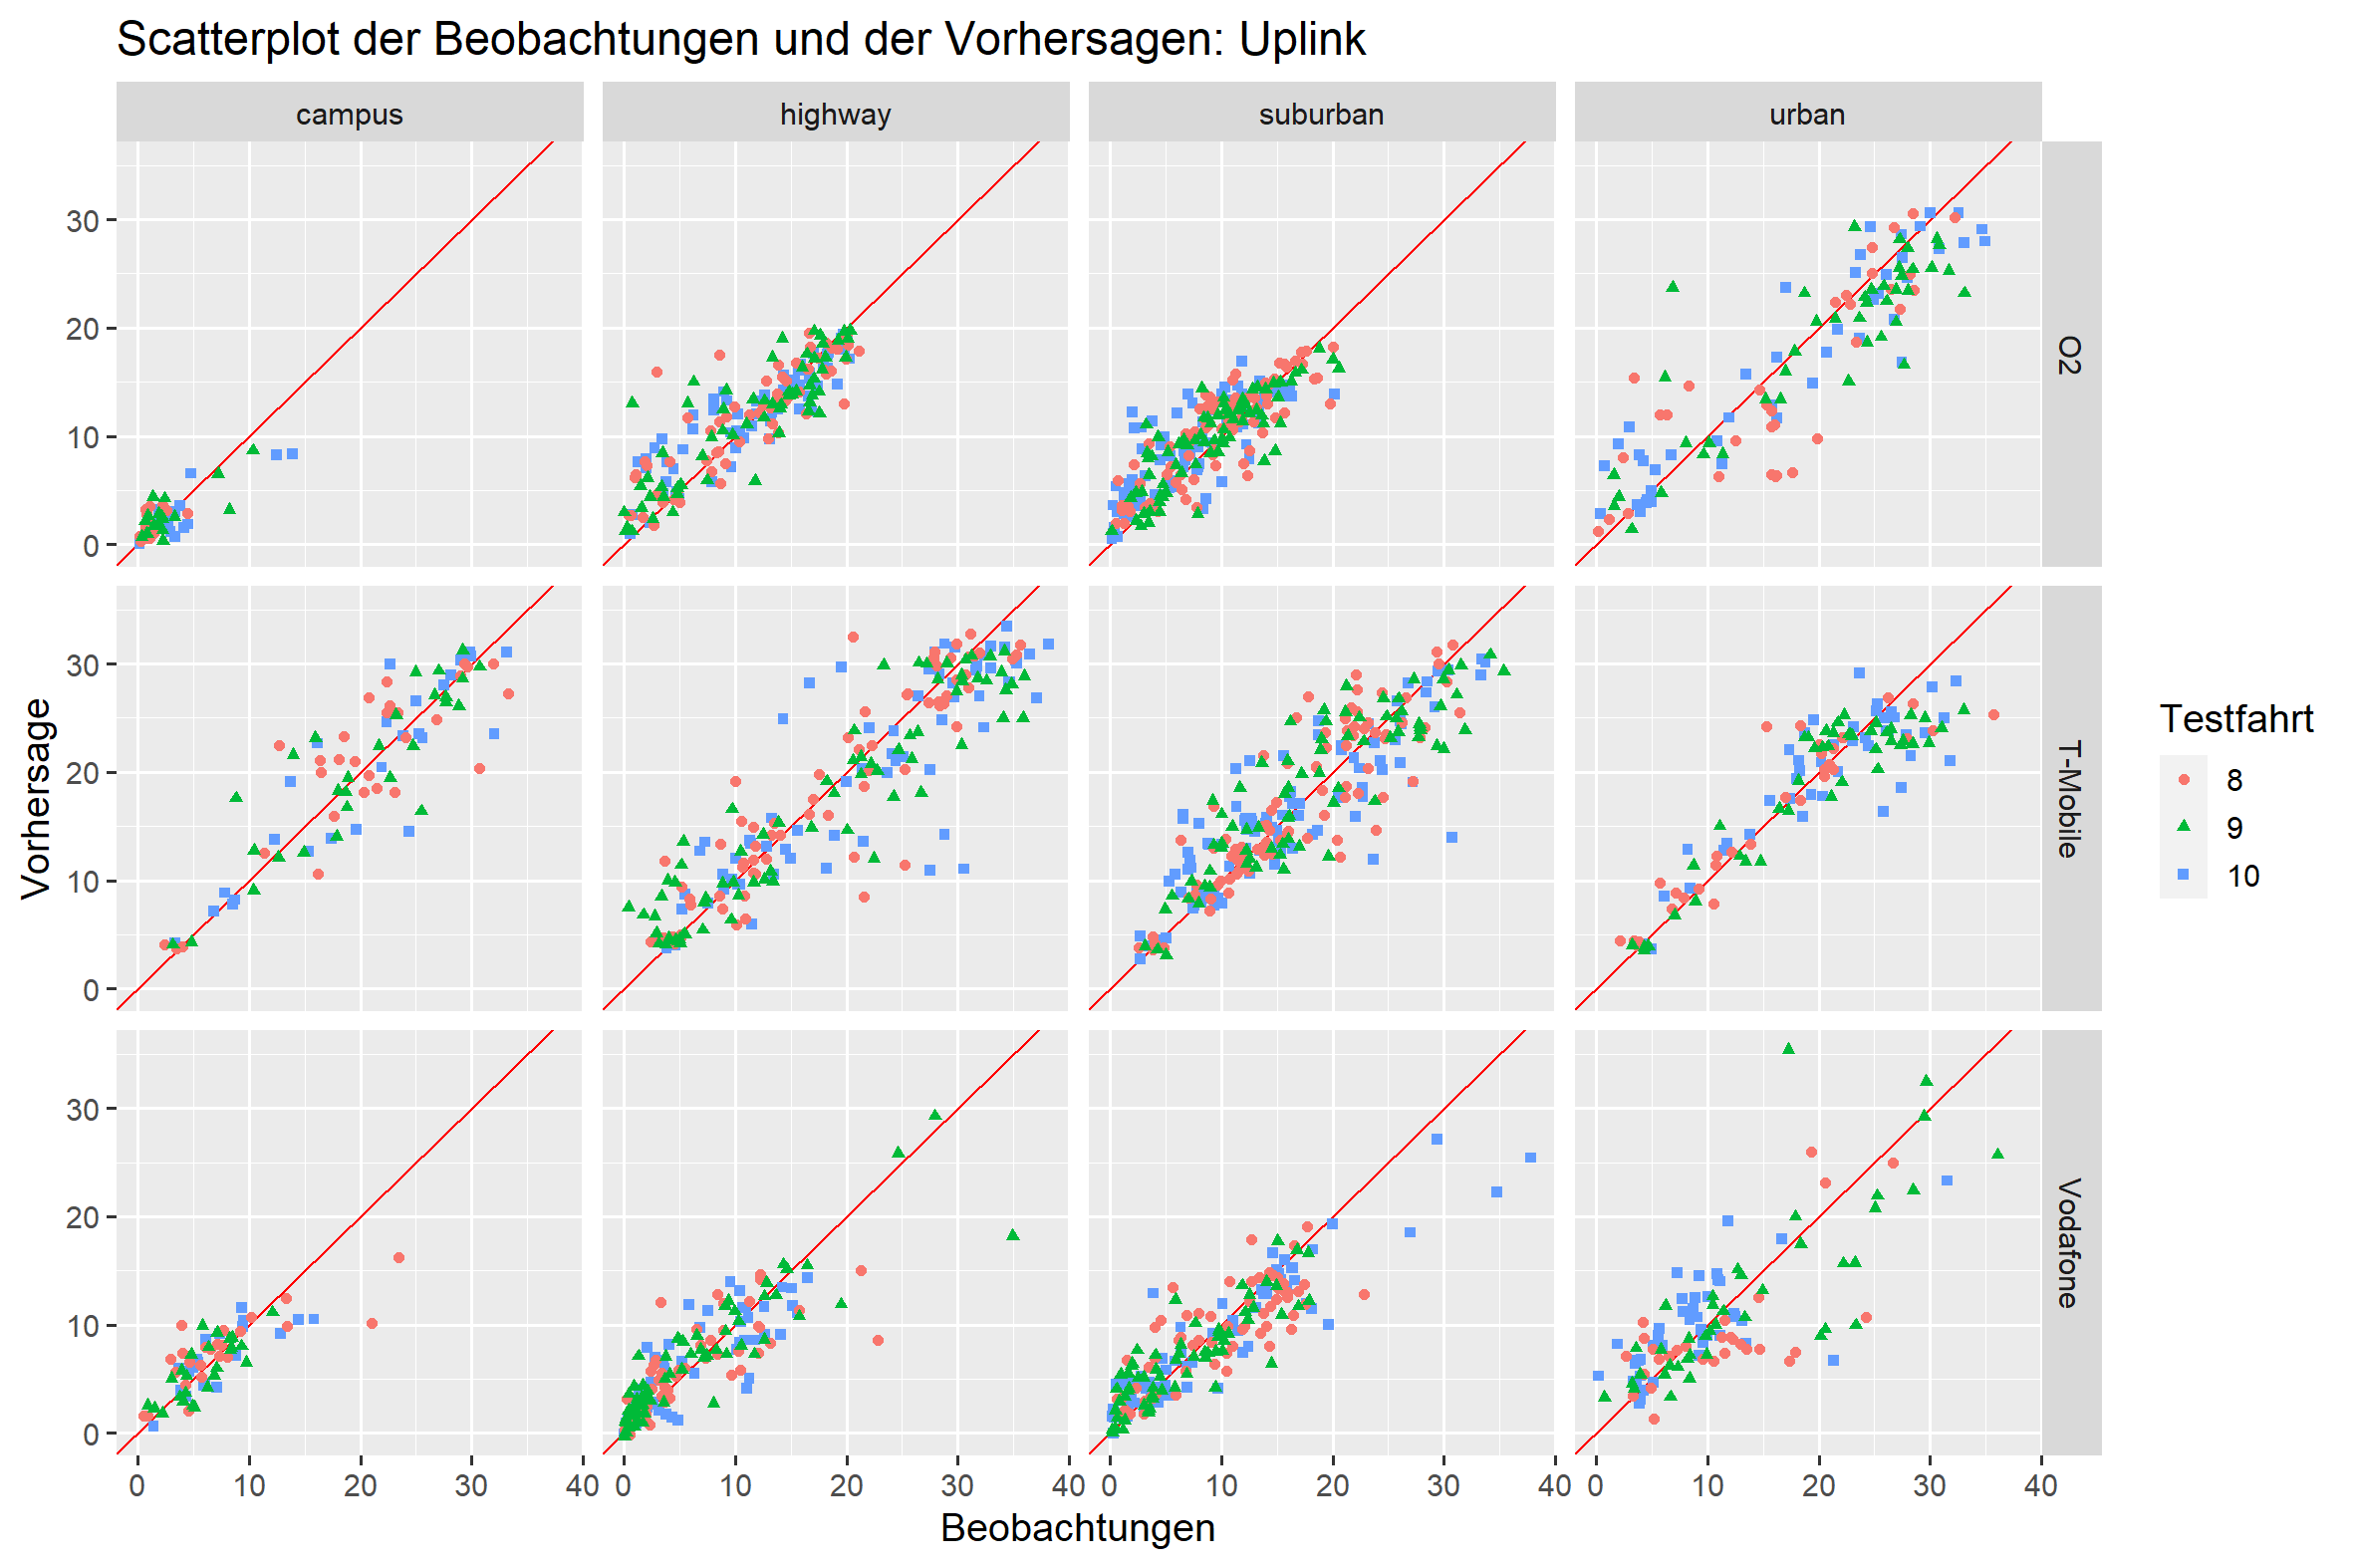
\includegraphics[width=\textwidth]{abbildungen/xgboost_predictions_ul}
\end{subfigure}
\begin{subfigure}{\textwidth}
    \centering
    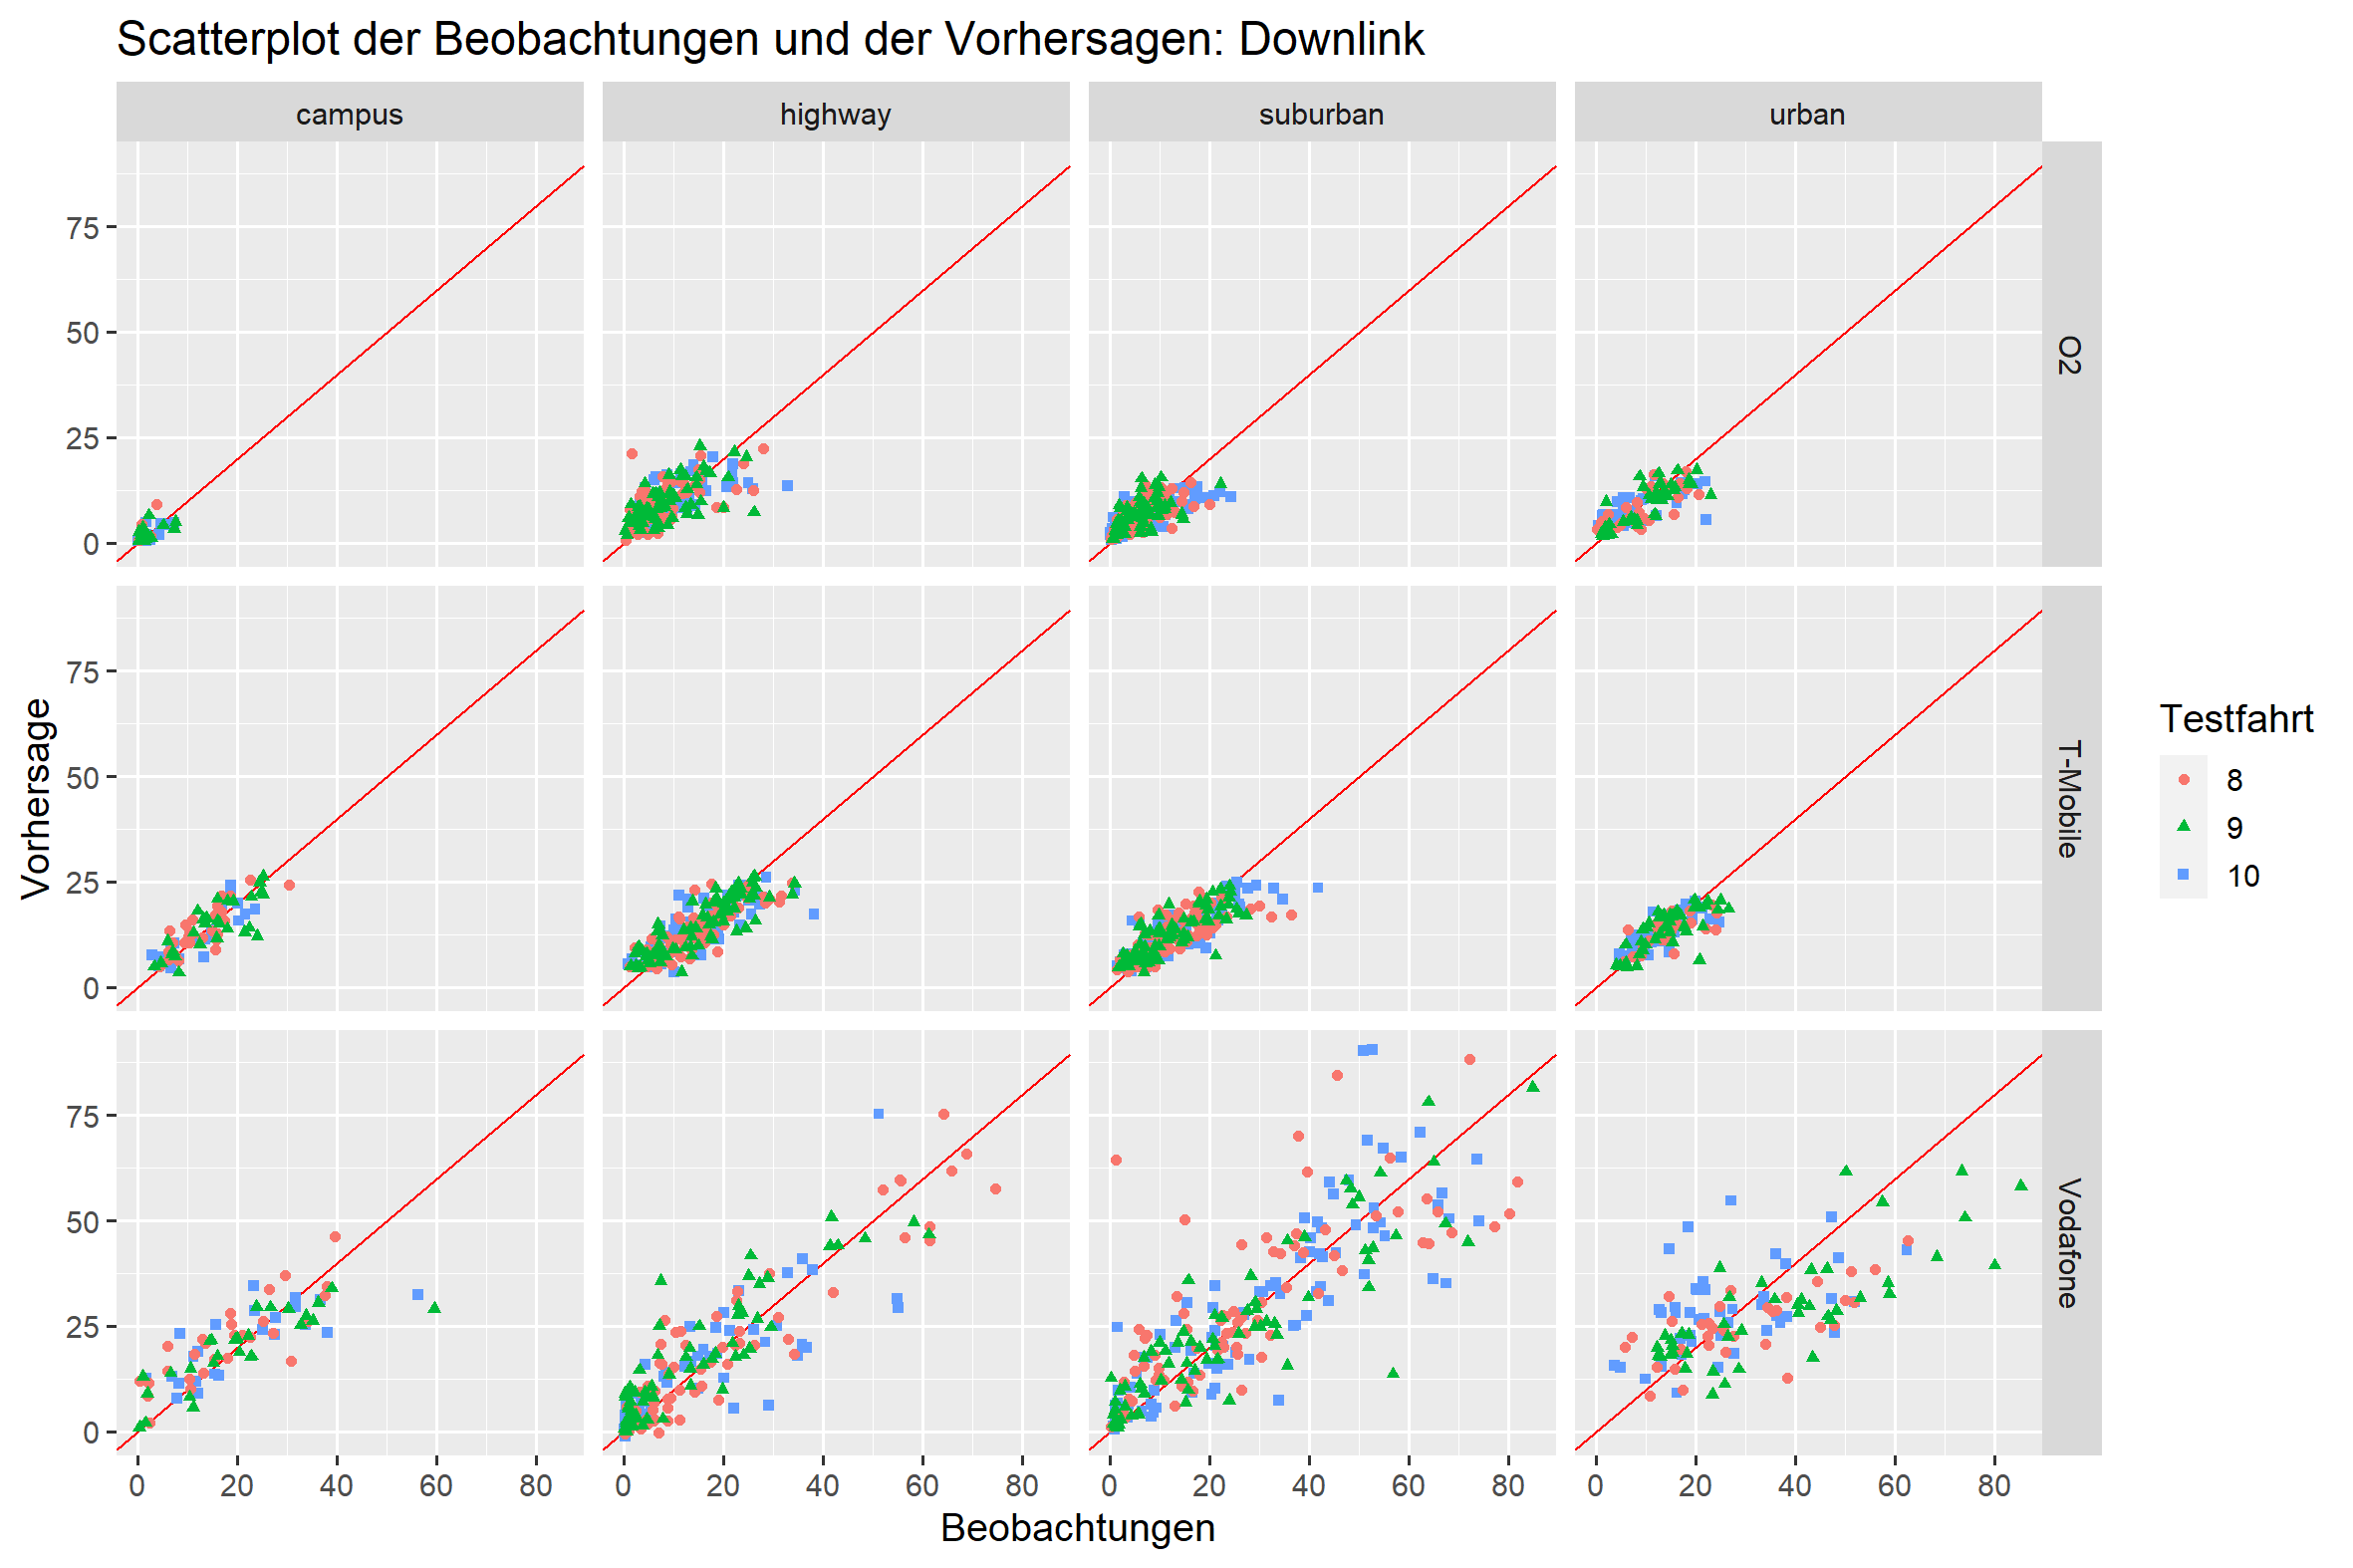
\includegraphics[width=\textwidth]{abbildungen/xgboost_predictions_dl}
\end{subfigure}
\caption{Out-of-Sample Vorhersagen der Datenraten f\"ur Extreme Gradient Boosting.}
\label{fig:datarate-predictions-xgboost}
\end{figure}

\subsubsection{Regression mit ARMA-Fehlern}

\begin{figure}
\centering
\begin{subfigure}{\textwidth}
    \centering
    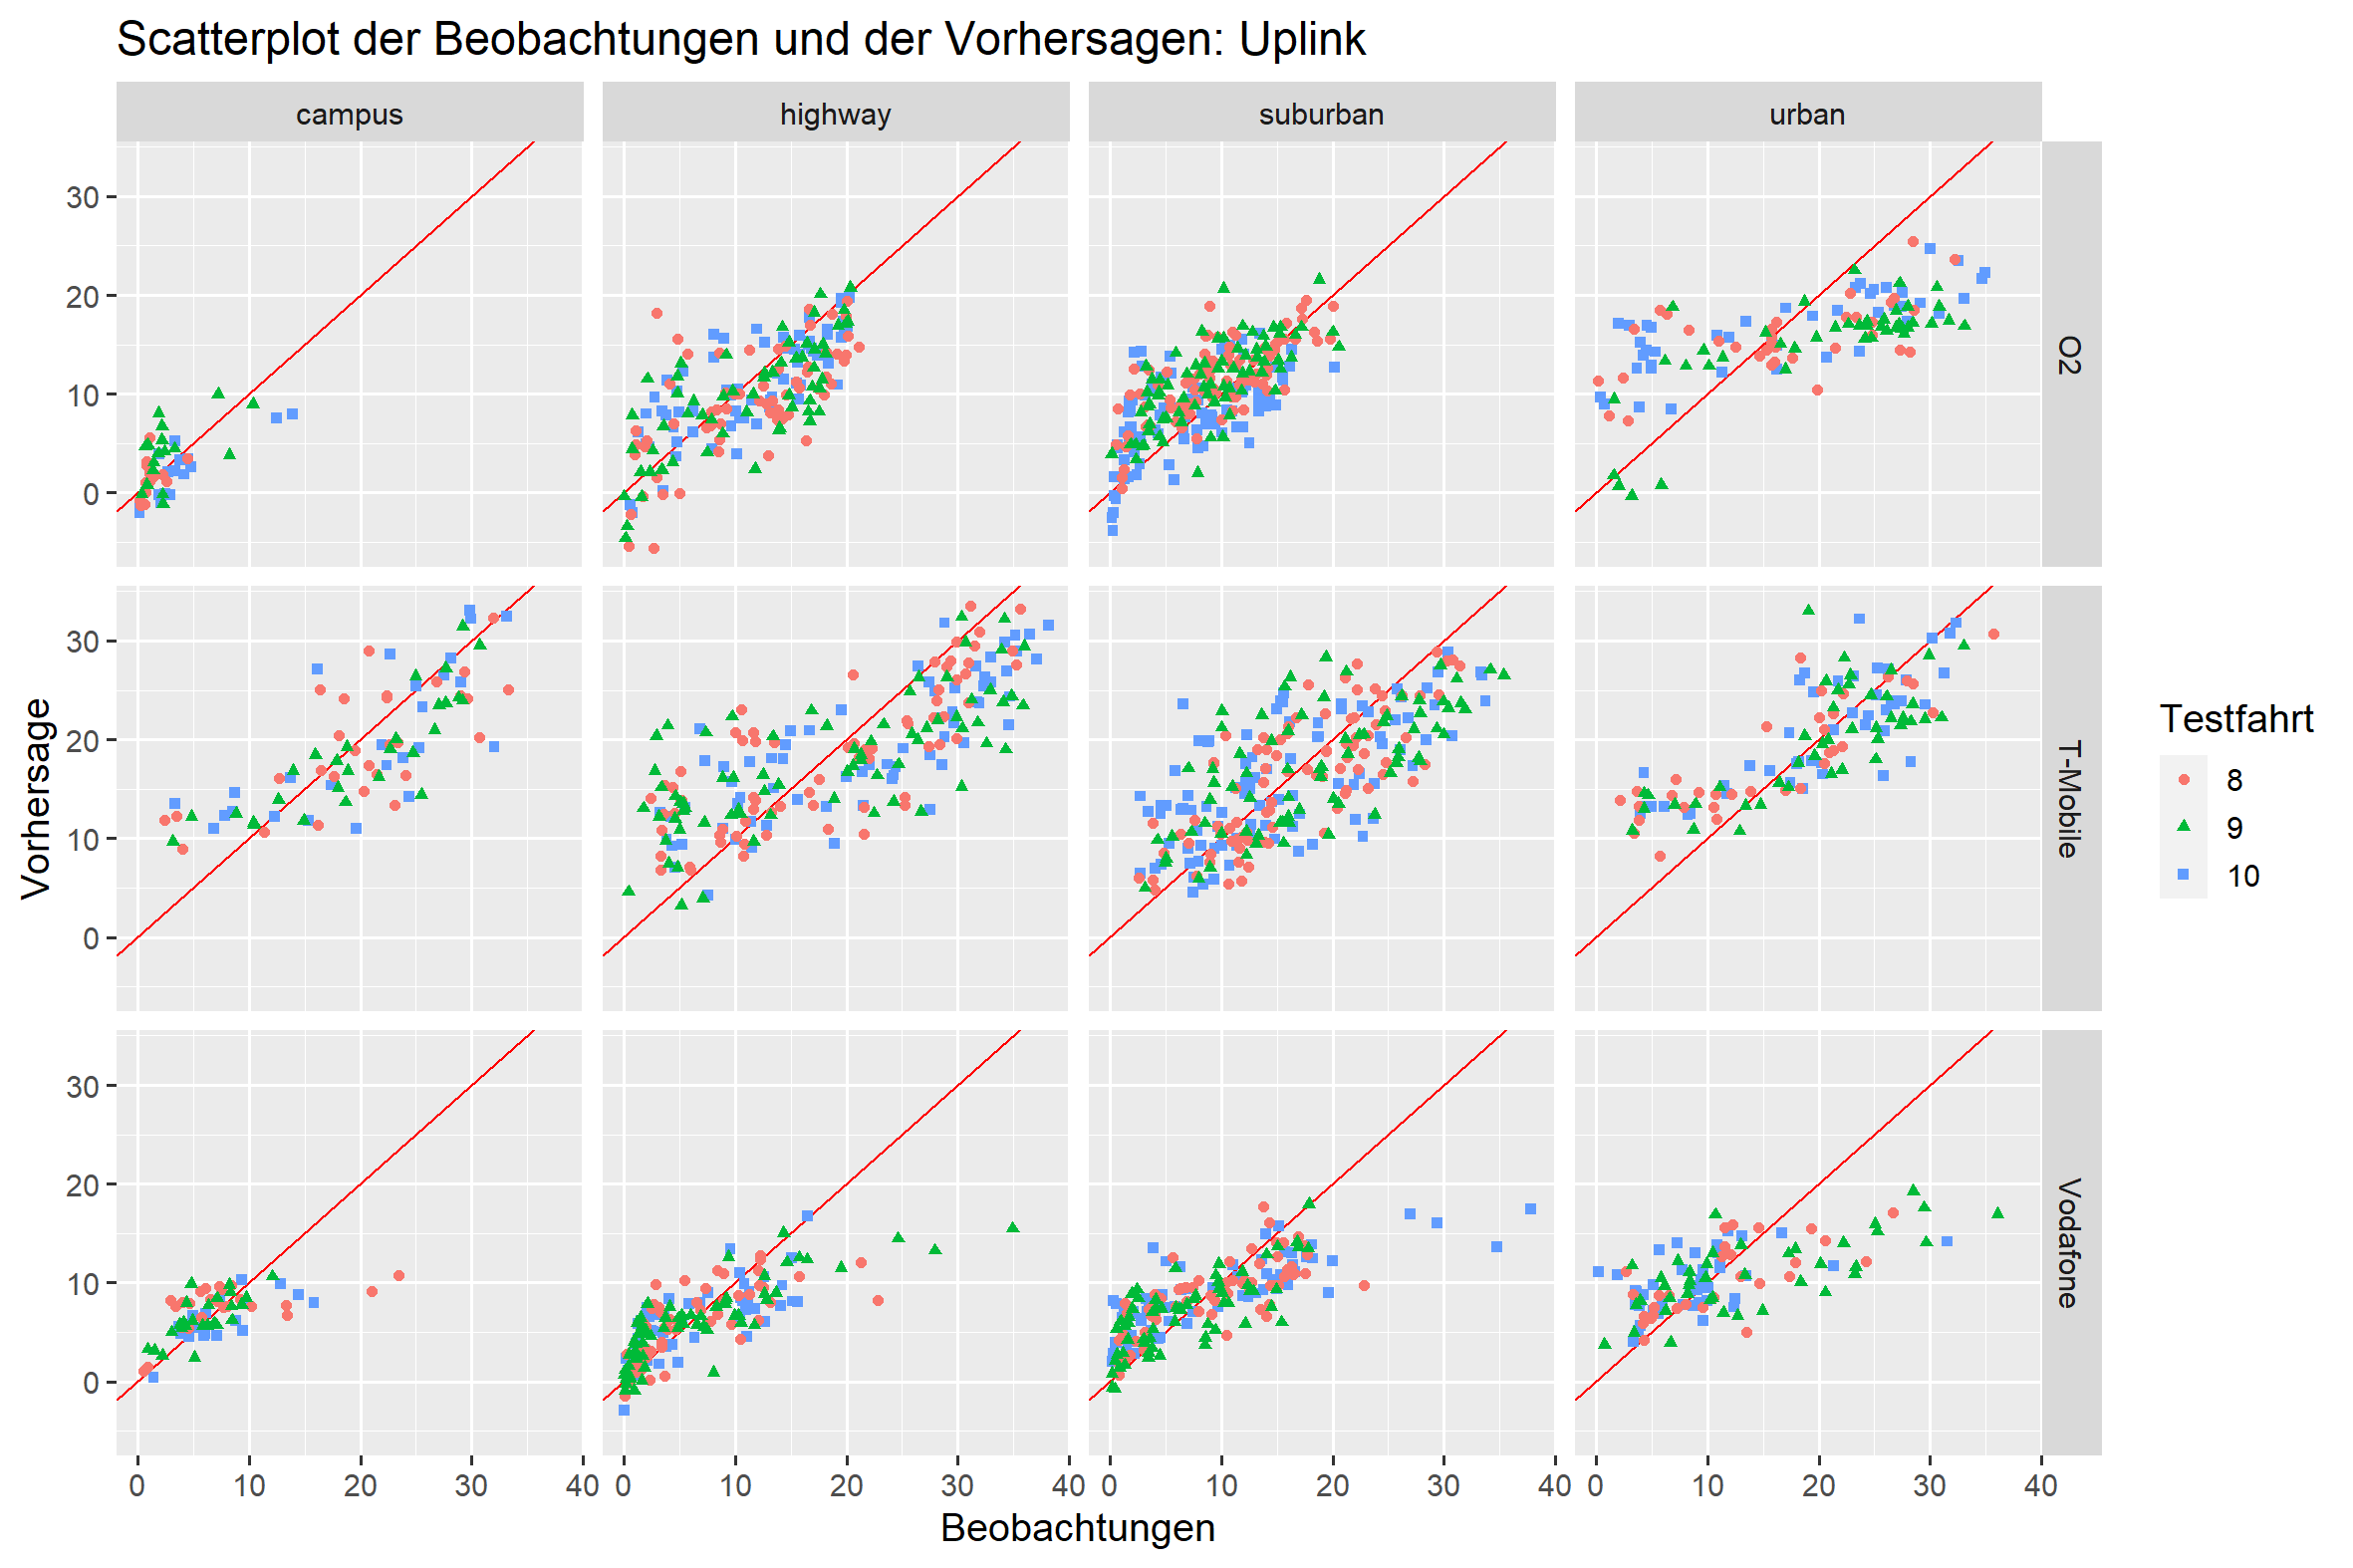
\includegraphics[width=\textwidth]{abbildungen/arma_predictions_ul}
\end{subfigure}
\begin{subfigure}{\textwidth}
    \centering
    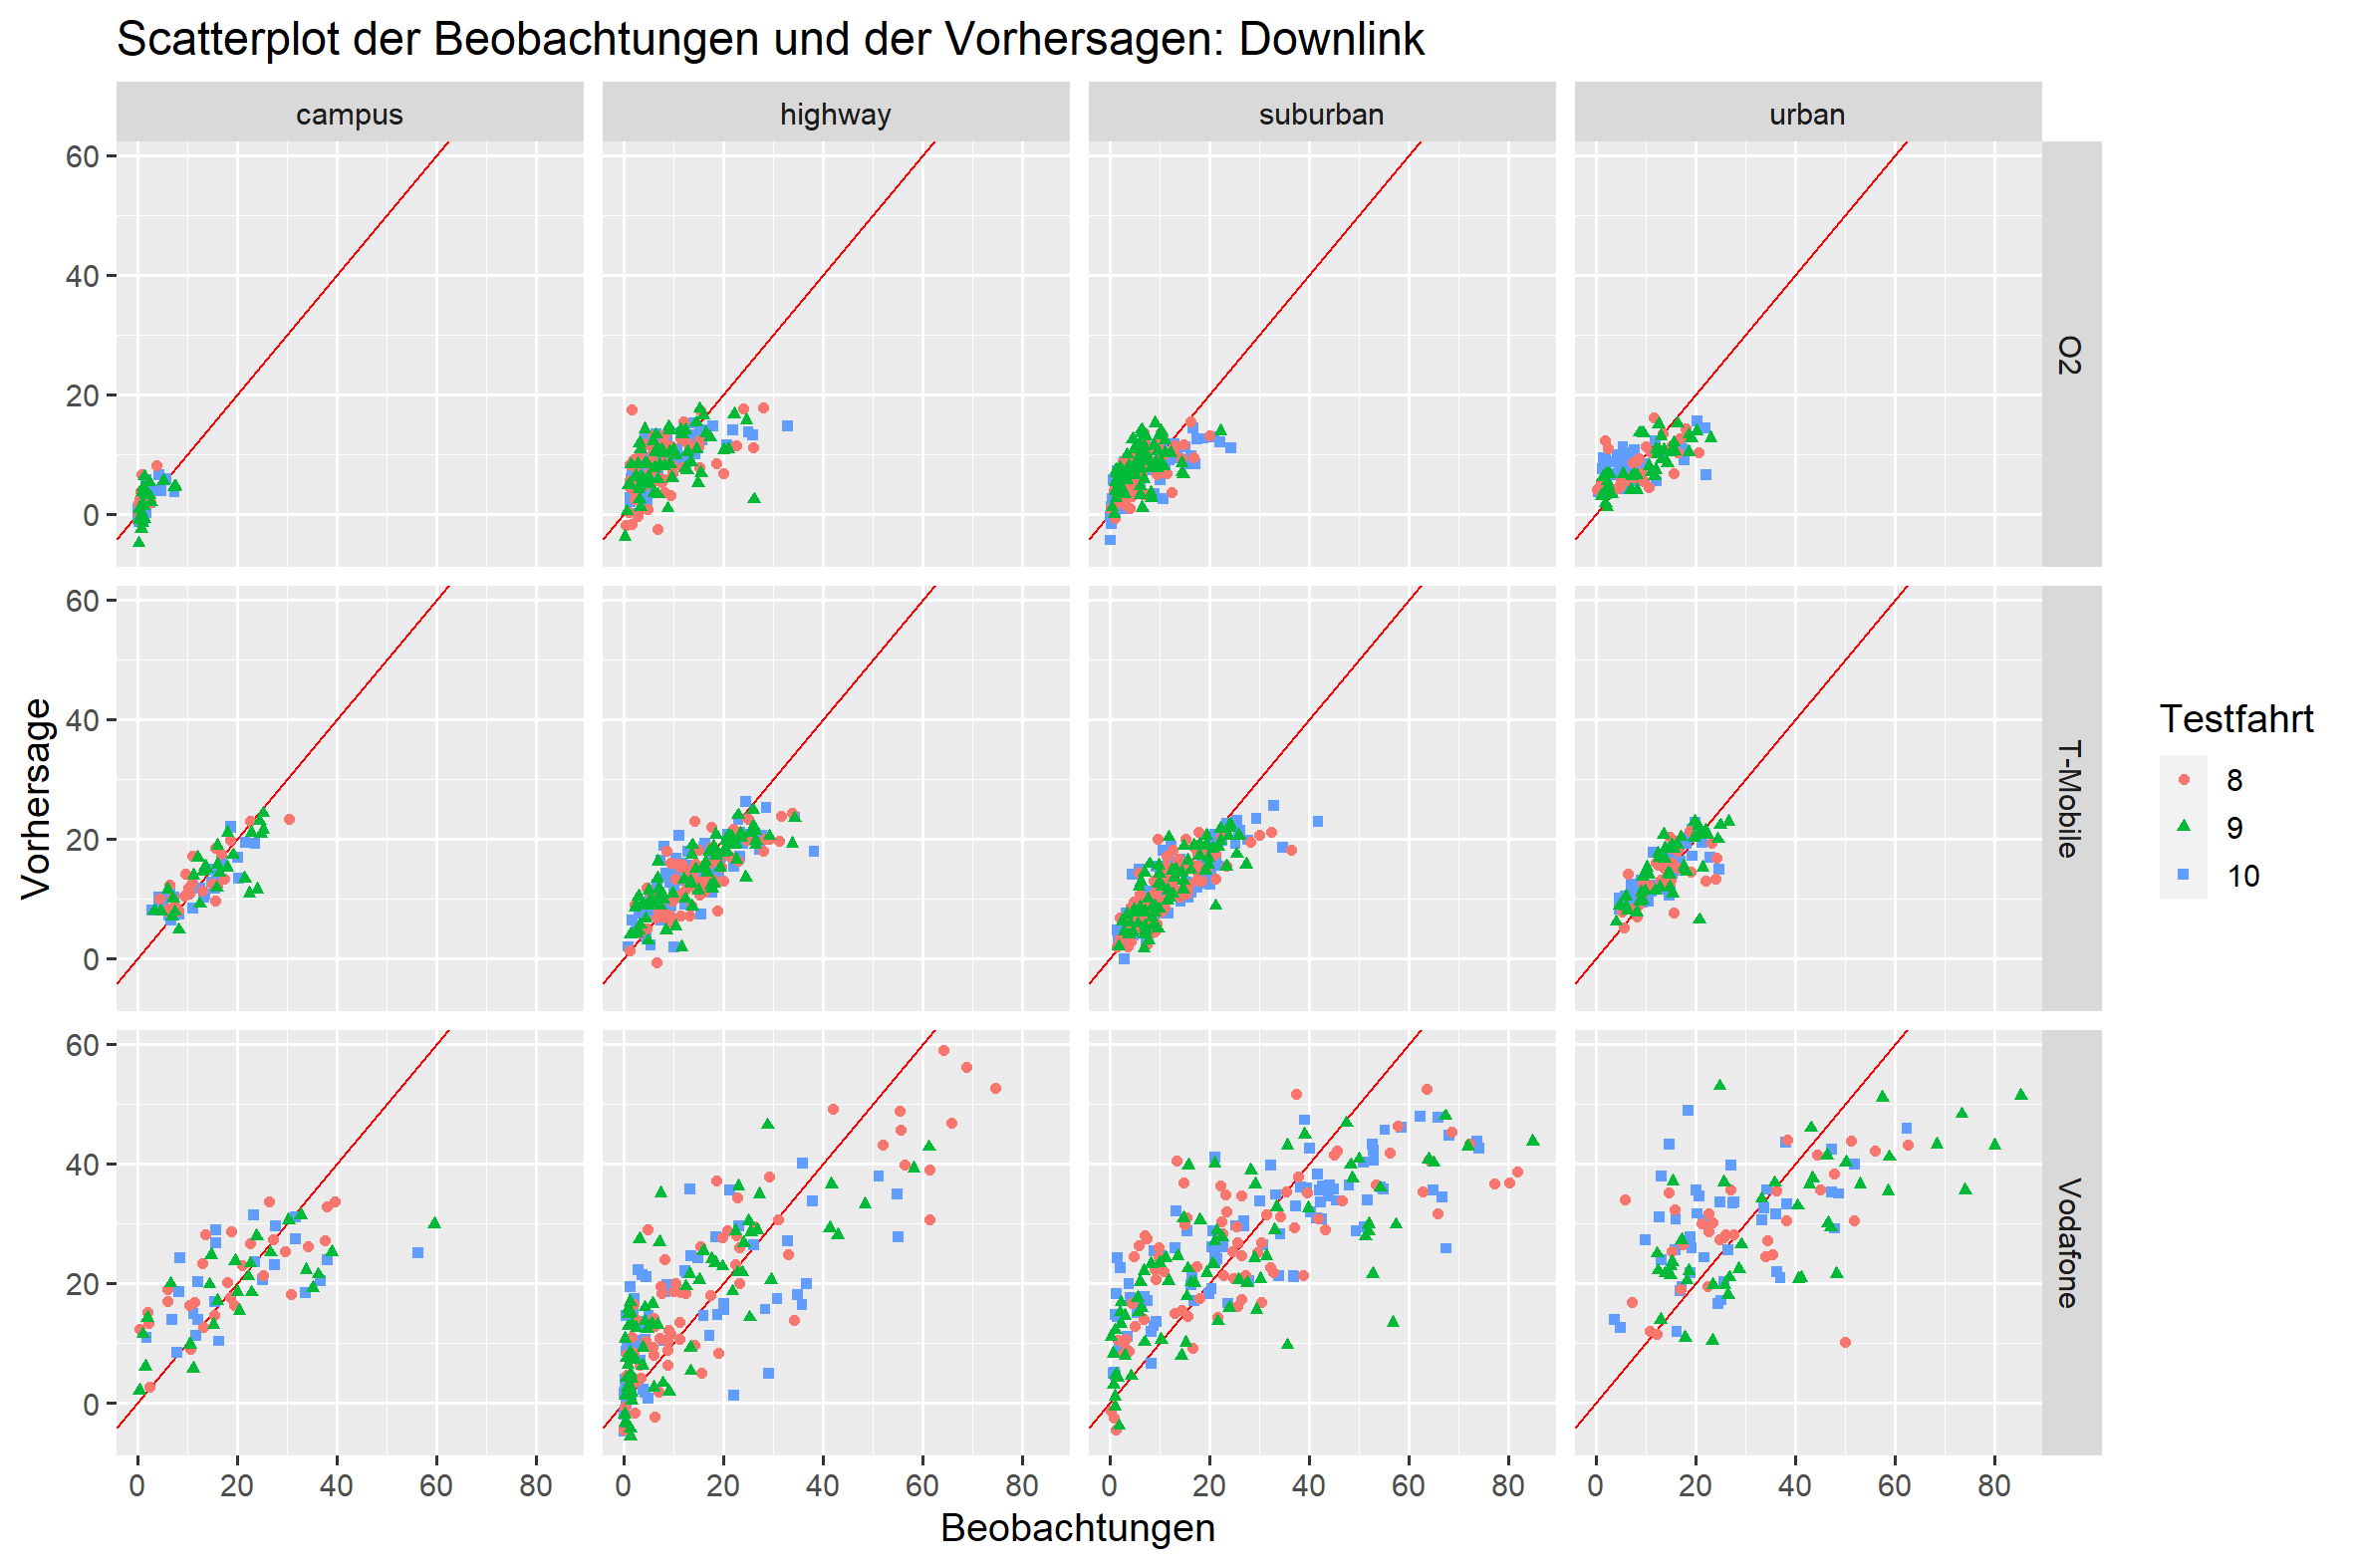
\includegraphics[width=\textwidth]{abbildungen/arma_predictions_dl}
\end{subfigure}
\caption{Out-of-Sample Vorhersagen der Datenraten f\"ur die Regression mit ARMA-Fehlern.}
\label{fig:datarate-predictions-arma}
\end{figure}

\subsubsection{Modellvergleich}

\begin{figure}
\centering
\begin{subfigure}{0.49\textwidth}
    \centering
    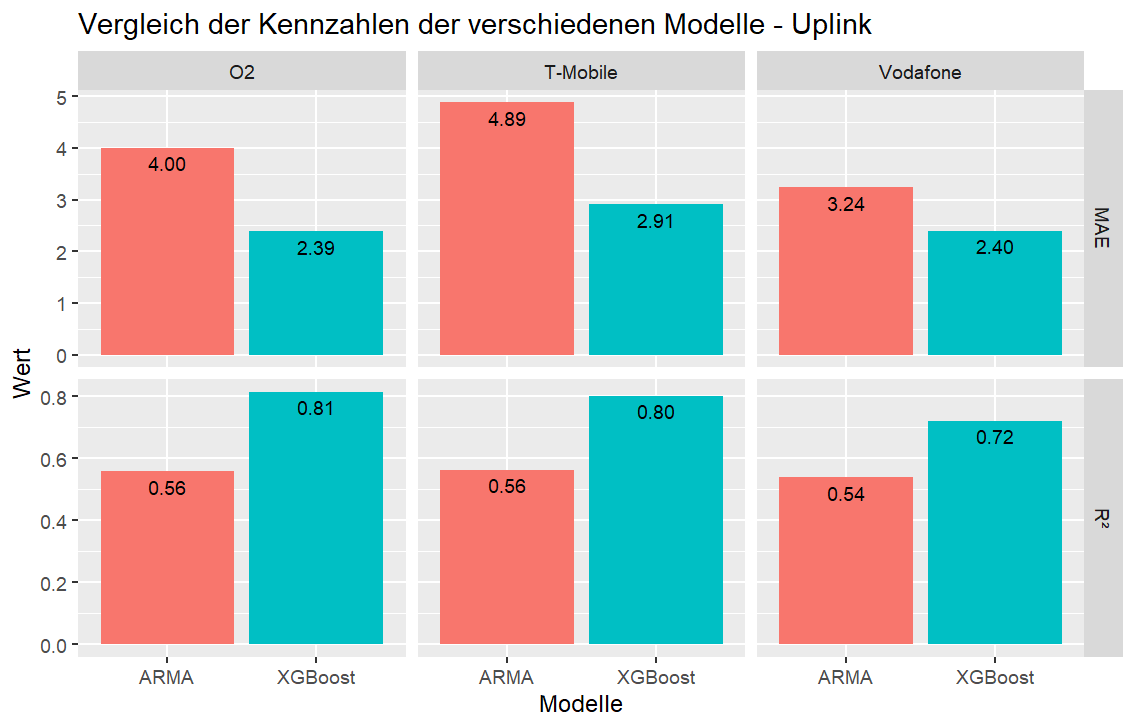
\includegraphics[width=\textwidth]{abbildungen/kennzahlen_vergleich_uplink}
\end{subfigure}
\begin{subfigure}{0.49\textwidth}
    \centering
    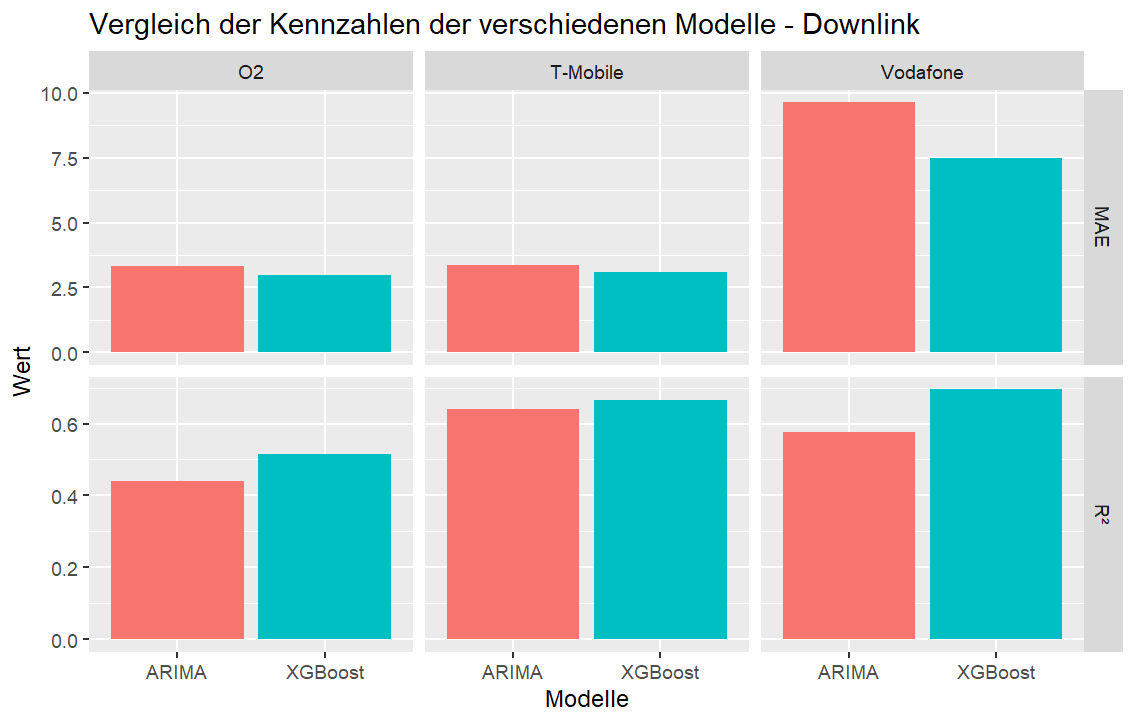
\includegraphics[width=\textwidth]{abbildungen/kennzahlen_vergleich_downlink}
\end{subfigure}
\caption{Vergleich der Kennzahlen f\"ur die Pr\"adiktion der Upload- und Download-Raten.}
\label{fig:kennzahlen-datarate}
\end{figure}

\begin{figure}
\centering
\begin{subfigure}{\textwidth}
    \centering
    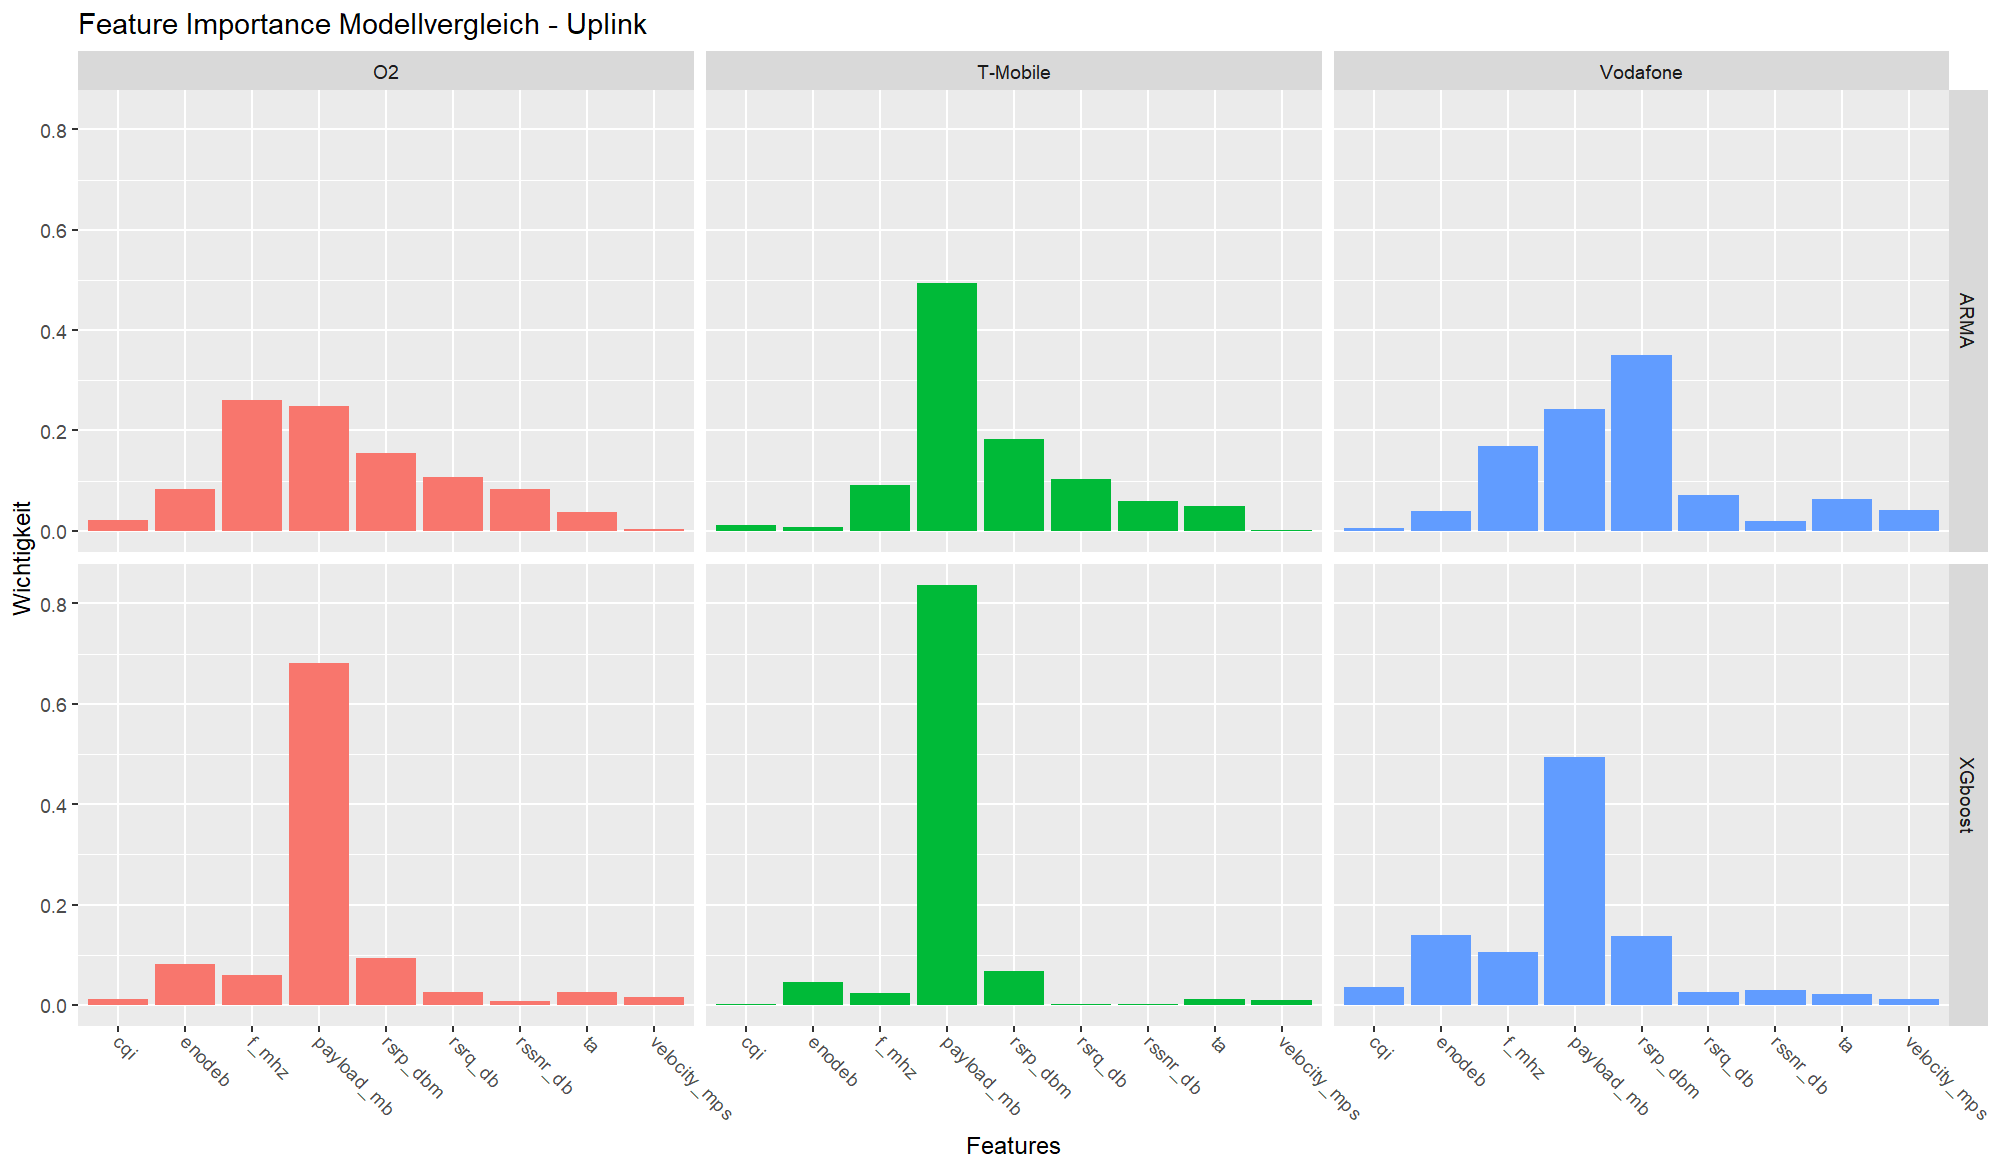
\includegraphics[width=\textwidth]{abbildungen/feature_importance_modellvergleich_uplink}
\end{subfigure}
\begin{subfigure}{\textwidth}
    \centering
    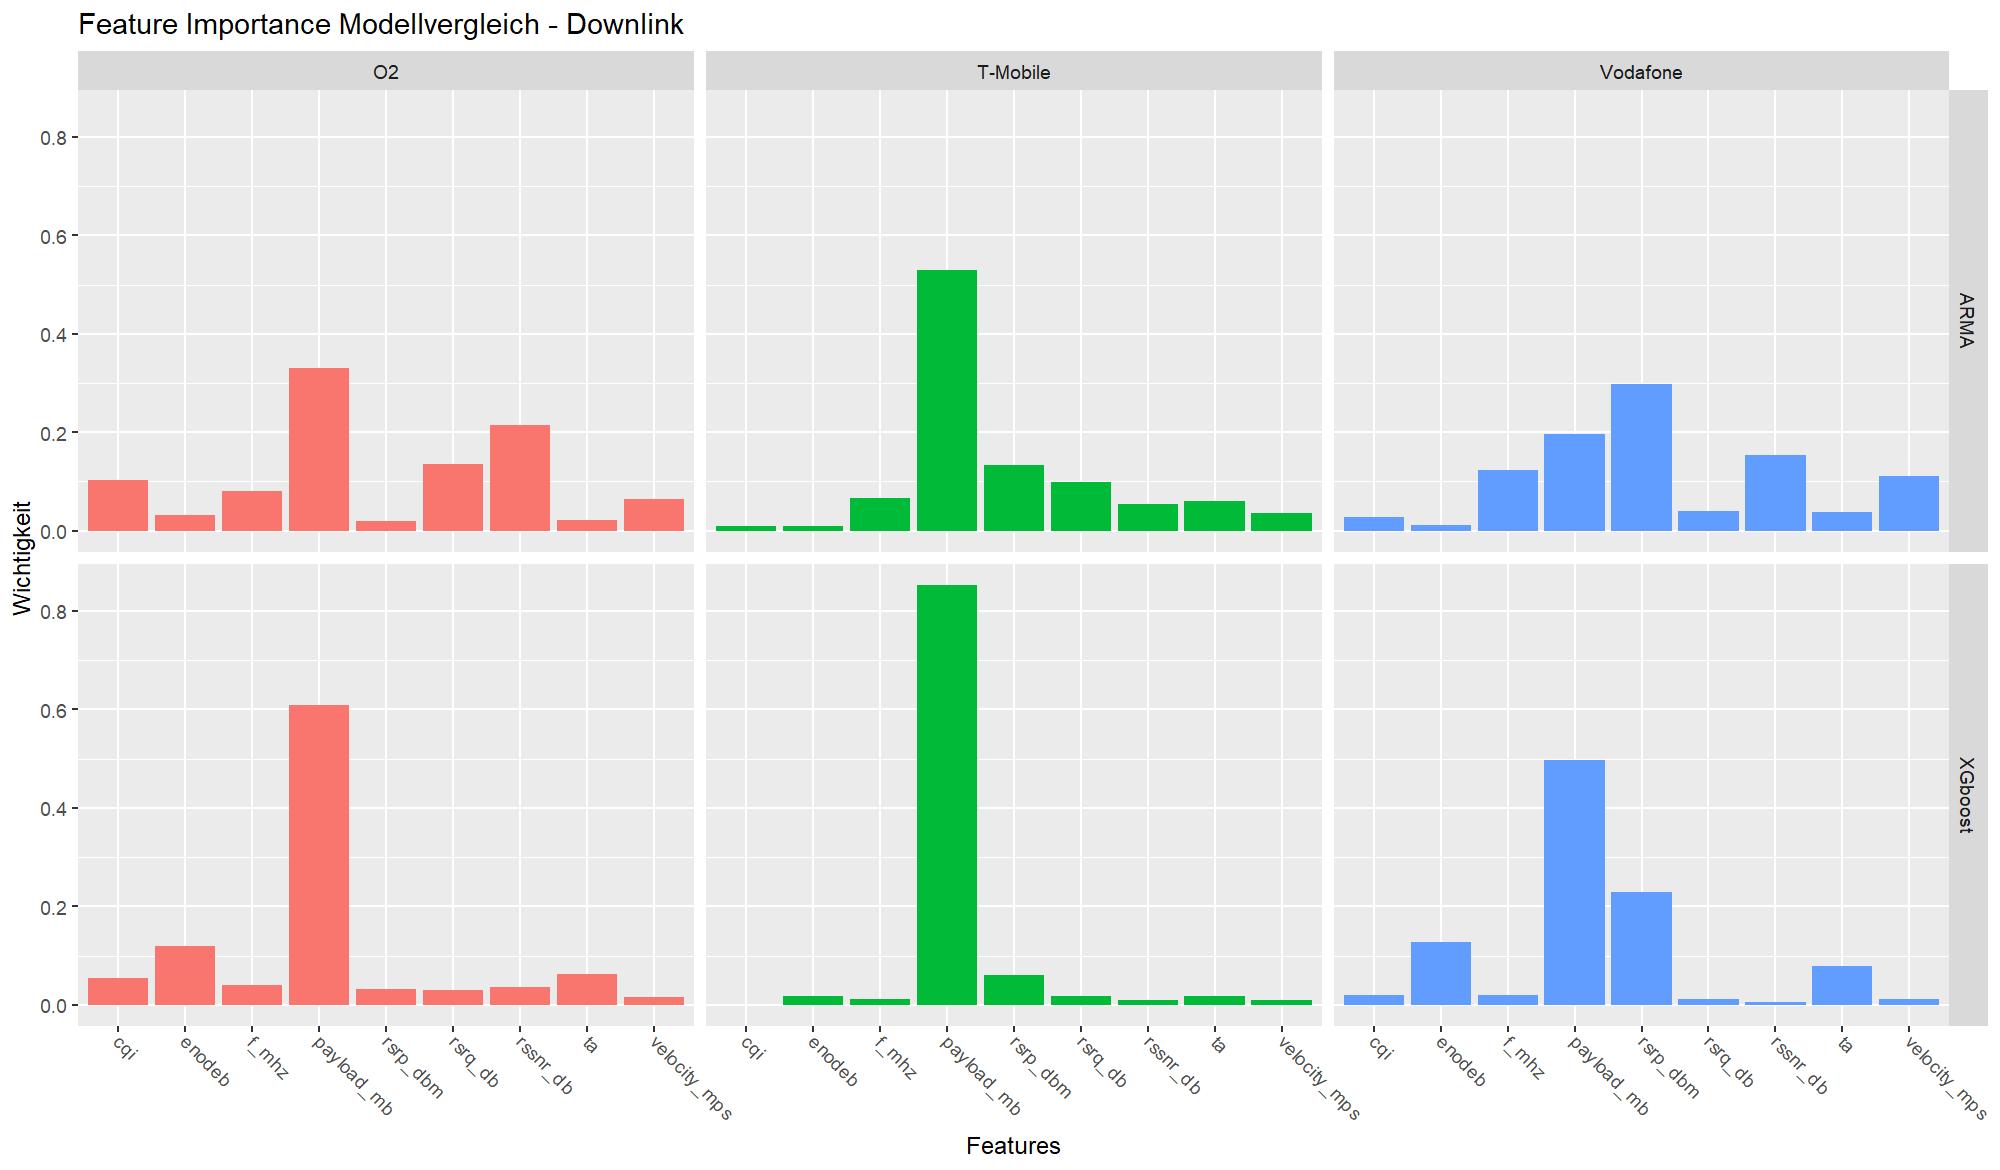
\includegraphics[width=\textwidth]{abbildungen/feature_importance_modellvergleich_downlink}
\end{subfigure}
\caption{Feature Importance der Modelle zur Datenratenpr\"adiktion.}
\label{fig:feature-importance-datenraten}
\end{figure}

\subsection{Vorhersage der eNodeB-Verbindungsdauern}

\begin{figure}
    \centering
    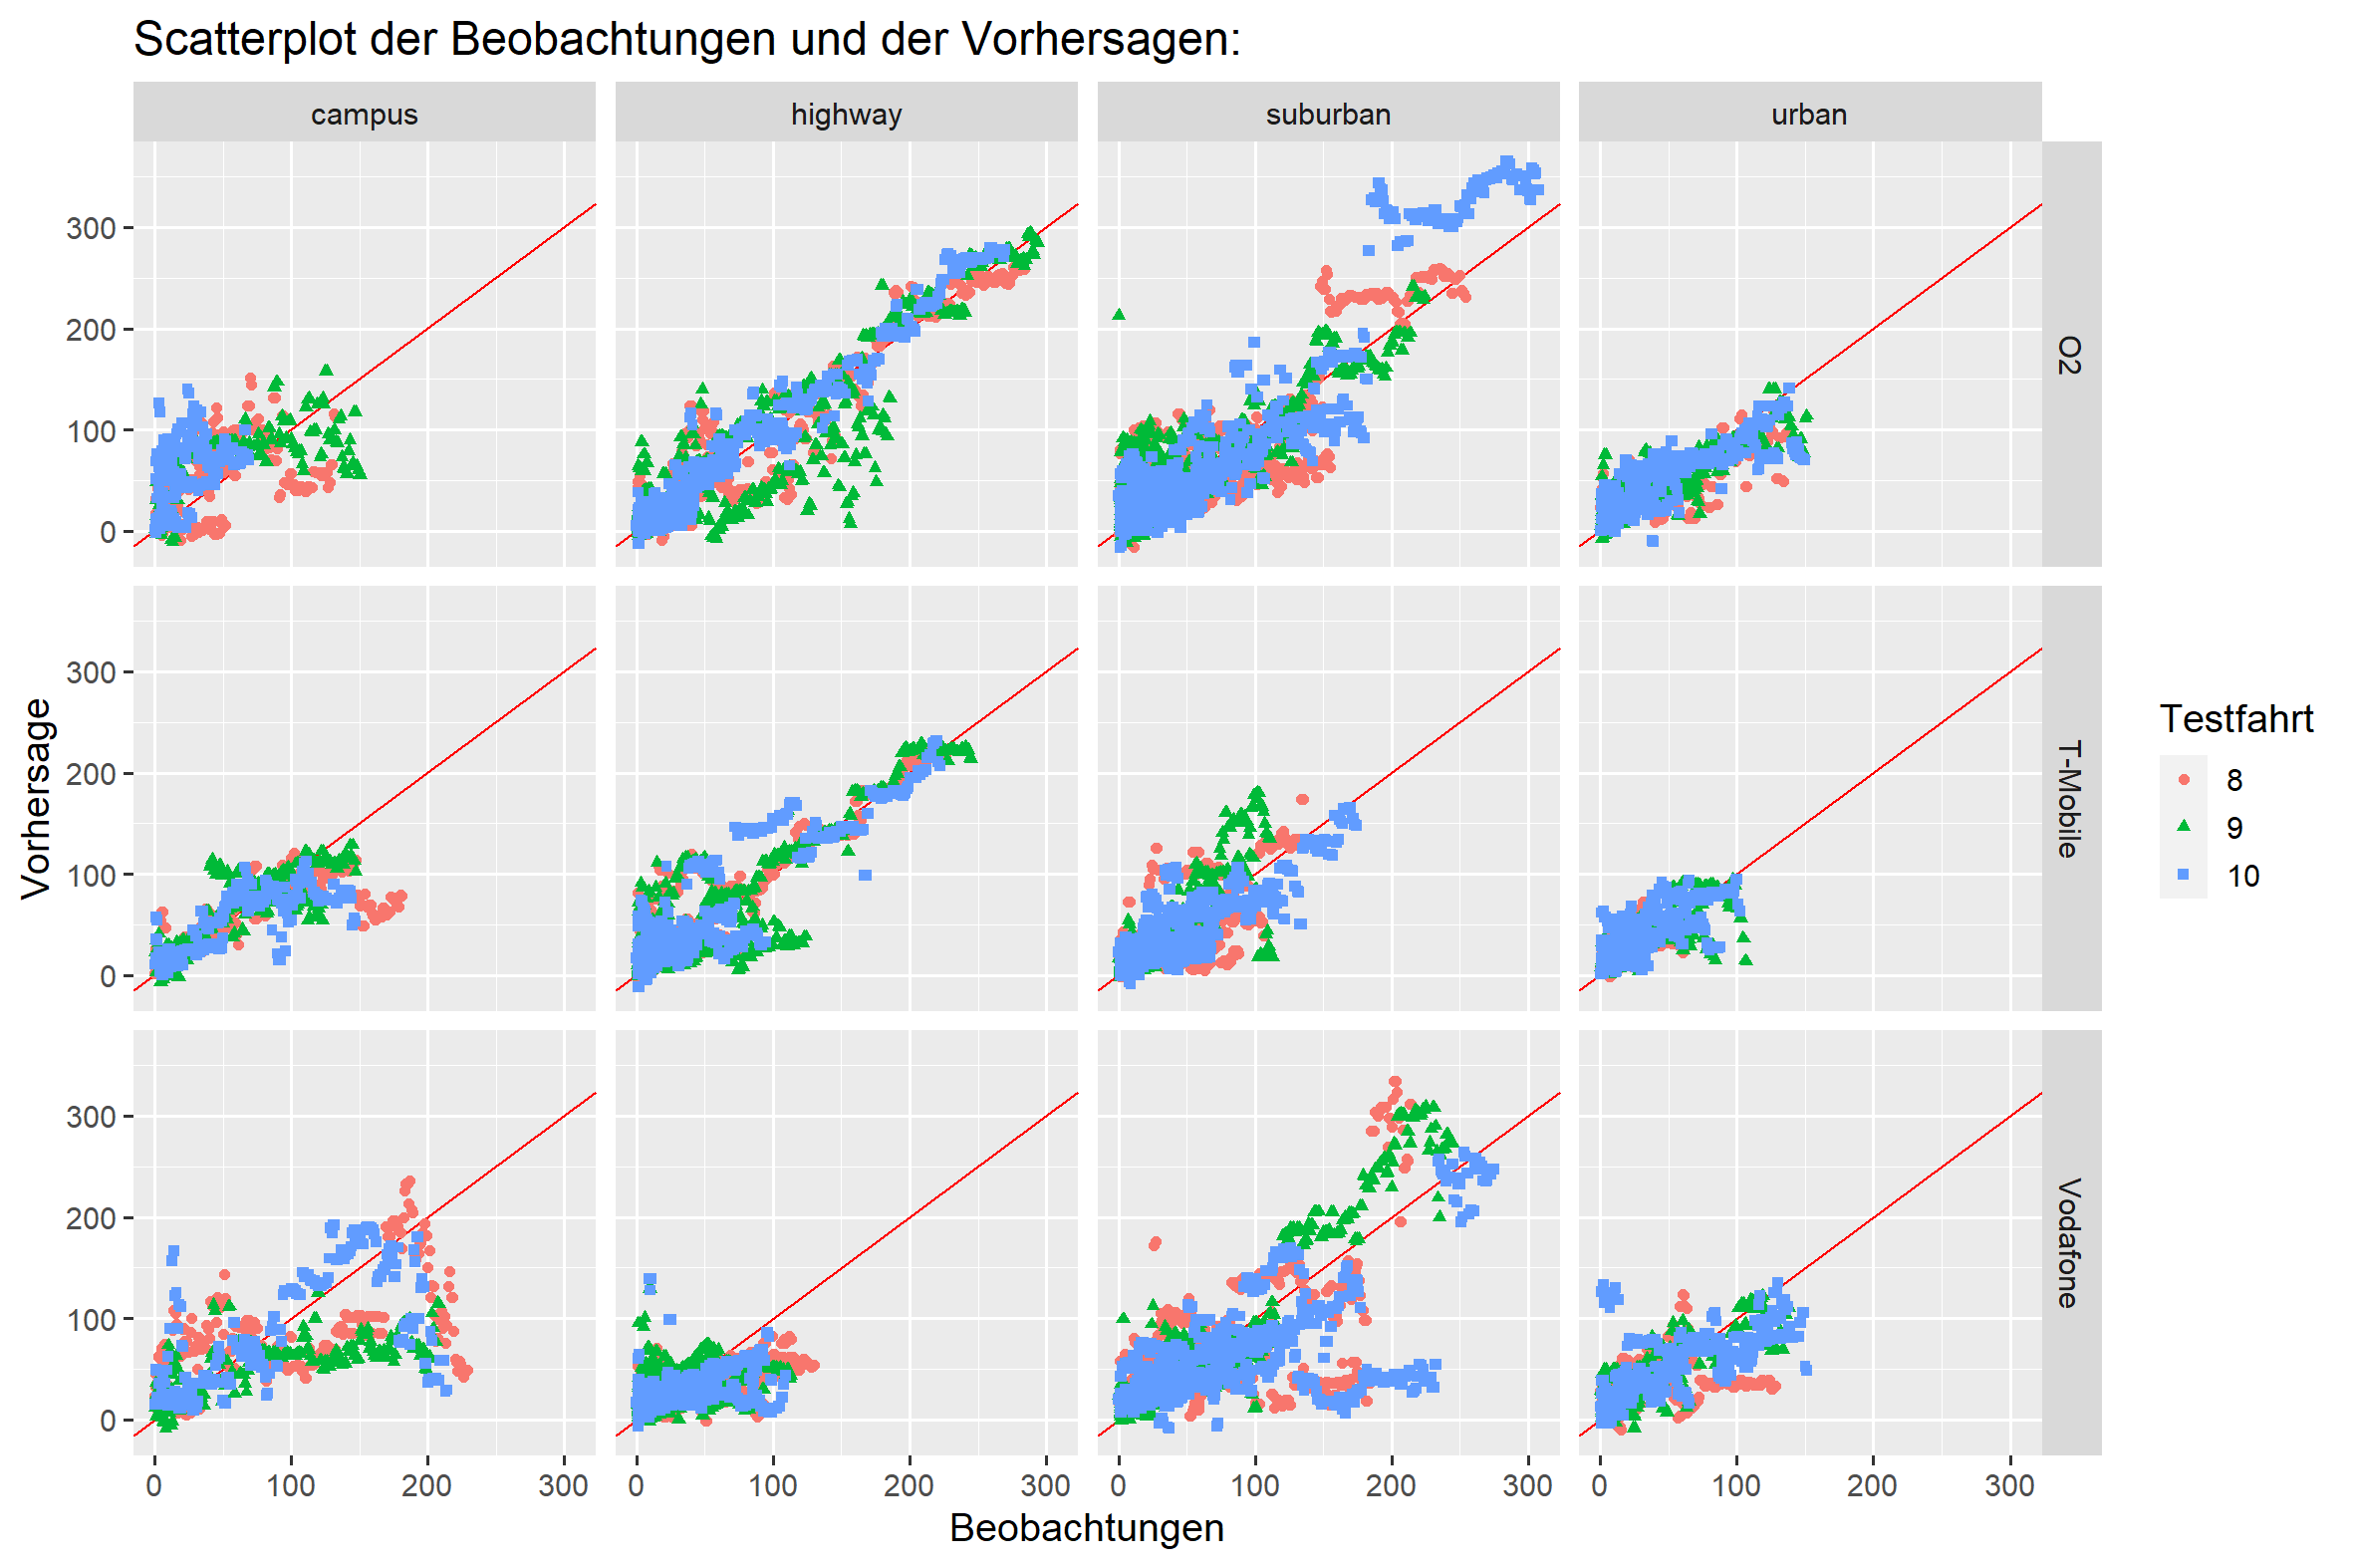
\includegraphics[width=\textwidth]{abbildungen/predictions_linklifetime}
    \caption{Out-of-Sample Vorhersagen der eNodeB-Verbindungsdauern.}
    \label{fig:link-lifetime-predictions}
\end{figure}

\section{Zusammenfassung}
\label{sec:zusammenfassung}

In diesem Projekt wurde gezeigt, wie das automatisierte Auslesen
von Nummernschildern aus Bilddaten mittels einer zweistufigen
Vorhersagepipeline umgesetzt werden kann.

In der ersten Stufe kam ein CNN zur Extraktion des Nummernschildes durch
Bildsegmentierung zum Einsatz.
Dieses neuronale Netz wurde so trainiert, dass es f\"ur jedes
Eingabebild eine bin\"are Maske vorhersagen sollte, in welcher
sich das Nummernschild befindet.
Zu diesem Zweck wurde der Trainings-Datensatz unter
Einsatz von Data-Augmentation Methoden von 949 auf 22776 Bilder
vergr\"o{\ss}ert.
Insgesamt zeigte der Einsatz des CNN zur Bildsegmentierung vielversprechende
Resultate: Auf einem Testdatensatz von 10 Bildern, die weder zum Training
noch zum early stopping verwendet wurden, konnte jedes der Nummernschilder
korrekt vom CNN erkannt werden. Selbst schwierige Lichtverh\"altnisse schienen
f\"ur das neuronale Netz kein Problem zu sein.

Anhand der Beispieldaten konnten allerdings keine Aussagen bez\"uglich
des Verhaltens auf rotierten Nummernschildern gemacht werden.
Zu dieser Situation lassen sich aber zwei \"Uberlegungen anstellen:
Zum einen wird durch Betrachtung der in~\ref{sec:Datenbeschreibung}
beschriebenen Trainingsdaten klar, dass die Kameras, welche ein Nummernschild
aufzeichnen, sehr h\"aufig so positioniert sind, dass das Nummernschild
achsenparallel zum Bildausschnitt verl\"auft. Die Rotationen, die in der
Praxis zu beobachten sind, scheinen also wenn \"uberhaupt nur recht
klein auszufallen. Man k\"onnte also einerseits argumentieren, dass
rotierte Nummernschilder in der Praxis nicht h\"aufig auftreten und dass
kleinere Rotationen immernoch hinreichend durch ein achsenparalleles
Rechteck erfasst werden k\"onnen.
Andererseits ist es so, dass sich der vorliegende Ansatz der
Berechnung eines umschlie{\ss}enden Rechtecks auch auf rotierte
Rechtecke verallgemeinern l\"asst. Am CNN m\"usste dazu nichts ge\"andert
werden, lediglich das Ausschneiden der Nummernschilder aus der
vorhergesagten bin\"aren Maske m\"usste
angepasst werden. Hierin best\"unde eine m\"ogliche zuk\"unftige
Verbesserung der ersten Stufe der Pipeline.

Die zweite Stufe der Pipeline, also die Zeichenerkennung aus einem
extrahierten Nummernschild, wurde mithilfe der OCR-Software Tesseract
unter Einsatz verschiedener Vorverarbeitungsschritte durch OpenCV realisiert.
Die Ergebnisse dieser Zeichenerkennung waren jedoch nicht
zufriedenstellend und m\"ussen noch verbessert werden.
In Abschnitt~\ref{sec:verbesserungen} wurden hierzu drei m\"ogliche
Ans\"atze diskutiert. Als letzter Ausweg wurde ein Wechsel der
Technologie hin zu CNNs zur Texterkennung in Betracht gezogen, wie sie
auch in~\cite{silva2018a} zum Einsatz kam. Es sollte
aber zun\"achst sichergestellt werden, dass die teils sehr
fehlerbehafteten Vorhersagen der Texterkennung nicht auf eventuelle
Implementierungsfehler zur\"uckzuf\"uhren sind, da sonst
m\"oglicherweise noch nicht das volle Potential der Tesseract Software
ausgenutzt wird.

Abschlie{\ss}end l\"asst sich jedoch feststellen, dass zumindest der erste Teil der
Pipeline erfolgreich umgesetzt wurde, was ein weiterer Beleg f\"ur die
Dominanz von CNNs im Bereich der Bildsegmentierung ist.
Die so umgesetzte Lokalisierung der Nummernschilder kann nun also
als solide Basis f\"ur alle weiteren Verbesserungen der
Texterkennung dienen.


\newpage

\nocite{*}

\bibliographystyle{plain}
\bibliography{literatur}

\end{document}